\documentclass[a4paper,12pt,twoside,BCOR=10mm]{scrbook}
% Packages
\usepackage{ucs}
\usepackage[utf8x]{inputenc}
\usepackage{t1enc}
\usepackage{graphicx}
\usepackage{enumerate,color}
\usepackage{url}
\usepackage[pdfborder={0 0 0}]{hyperref}
\usepackage{appendix}
\usepackage{eso-pic}
\usepackage{amsmath}
\usepackage{amssymb}
\usepackage[nottoc]{tocbibind}
\usepackage[sort&compress,authoryear]{natbib}
\usepackage[sf,normalsize]{subfigure}
\usepackage[format=plain,labelformat=simple,labelsep=colon]{caption}
\usepackage{placeins}
\usepackage{tabularx}
% Configurations
\graphicspath{{figs/}}

\setlength{\parskip}{\baselineskip}
\setlength{\parindent}{0cm}
\raggedbottom
% \setkomafont{subsection}{\normalfont\sffamily}

% Eins og templatið á að vera
% \setkomafont{captionlabel}{\itshape}
% \setkomafont{caption}{\itshape}

% Mun fallegri lausn
\setkomafont{captionlabel}{\itshape}
\setkomafont{caption}{\itshape}
\setkomafont{section}{\FloatBarrier\Large}
\setcapwidth[l]{\textwidth}
\setcapindent{1em}


% Times new roman
\usepackage[T1]{fontenc}
\usepackage{mathptmx}

%%%%%%%%%%% MODIFY THESE LINES ONLY %%%%%%%%%%%%%%%%%%%%%%%%%%%%%%%%%%%%%%%%%%%%%%%%%%%%%%%%%
\def\thesisyear{2014}       						% Year thesis submitted
\def\thesismonth{}						% Month thesis submitted
\def\thesisauthor{}					% Thesis authoreiningaraðferðinni
\def\thesistitle{Matemática para a Computação} 						% Title of thesis
\def\thesisshorttitle{Introdução ao Cálculo} 	% Title of thesis
\def\thesiscredits{XX} 							% Credits awarded for the project
\def\thesissubject{XX}
\def\thesiskind{}							% Masters of PhD thesis
\def\thesiskindformal{}				% Masters of PhD thesis
\def\thesisnroftutors{1}						% Number of tutors
\def\thesisschool{School of Engineering and {Natural Sciences}}		% School
\def\thesisfaculty{XX}							% Faculty
\def\thesisaddress{XXFaculty street address}				% Office address
\def\thesispostalcode{XXFaculty postal code, Reykjavik}			% Office address
\def\thesistelephone{525 4000}						% Office telephone
\def\thesispublisher{XX}						% Publisher
\def\thesistutors{XXNN1 \\ XXNN2}
\def\thesisrepresentative{XXNN3}					% Tutors name
\def\thesiscommittee{XXNN4 \\ XXNN5 }
\def\thesiskeywords{Keyword1, Keyword2, Keyword3}			% Keywords
\def\thesisISBN{XX}           						% Thesis ISBN number
\def\thesisdedication{Dedication}
\def\thesisPrinting{Háskólaprent, Fálkagata 2, 107 Reykjavík}

% Function to add footer to frontpage
\newcommand\BackgroundPic{
\put(0,0){
\parbox[b][\paperheight]{\paperwidth}{
\vfill
\centering
\hspace*{-0.6cm}
%\includegraphics[width=\paperwidth,height=\paperheight,
%keepaspectratio]{foot}

\includegraphics[width=\paperwidth,height=\paperheight,
keepaspectratio]{HI.jpeg}
}}
\setlength{\unitlength}{\paperwidth}
\begin{picture}(0,0)(0,-0.15)
\put(0,0){\color{white}\parbox{1\paperwidth}{\centering\bfseries\sffamily \Large
Universidade Federal de Pelotas\\
\thesisyear}}
\end{picture}
}

\begin{document}

\begin{titlepage}
\thispagestyle{empty}
\AddToShipoutPicture*{\BackgroundPic}
%
\begin{center}
\vspace*{1cm}
%\includegraphics[width=43.6mm]{ui_1_cmyk}\\

\includegraphics[width=43.6mm]{aUI.png}\\
\vspace*{3.0cm}
\huge \sffamily \bfseries \thesistitle

\vspace*{5.5cm}
\normalfont \Large \sffamily \thesisauthor
\AddToShipoutPicture*{\BackgroundPic}
\vfill

\end{center}
\newpage

%PAGINA DOS OBJETIVOS DA OFICINA
\setcounter{page}{5}
\section*{\huge Prefácio}
Frequentemente, os alunos ao ingressarem em um curso que envolve o estudo de tecnologia, como o Bacharelado em Ciência da Computação e Engenharia de Computação, possuem uma enorme expectativa de estudos com disciplinas práticas e tecnológicas. A maioria dos alunos ingressantes não tem a idéia da carga de disciplinas teóricas e formais que esses cursos possuem. Assim, à medida que deparam com tais disciplinas, acabam por considerar como um estudo secundário, ou algo que não será tão relevante para sua formação.

Mesmo que o professor enfatize a importância das disciplinas teóricas e matemáticas para a formação do aluno, ou mesmo que ele relacione o conteúdo ministrado com outras disciplinas que serão estudadas ao longo do curso, o aluno tende a não dar a devida importância ou até mesmo esquece rapidamente do que foi trabalhado ao longo do semestre. 

As disciplinas teóricas mais importantes, e que geram maior reprovação e evasão, para os cursos de Ciência da Computação e Engenharia de Computação são Sistemas Discretos e Cálculo Diferencial e Integral, onde os conteúdos ministrados são essenciais e fundamentais para várias outras disciplinas ao longo do curso, tais como: Banco de Dados, Algoritmos, Estrutura de Dados, Técnicas Digitais, Análise de Algoritmos, Teoria da Computação, entre outras.

\vfill \vspace*{1cm}

\tableofcontents

\chapter{Conjuntos}
\pagenumbering{arabic}
\setcounter{page}{1}
A Teoria dos conjuntos  é a teoria matemática dedicada ao estudo da associação entre objetos, elaborada por volta do ano de 1872. Sua origem pode ser encontrada nos trabalhos do matemático russo Georg Cantor (1845-1918), os quais buscavam a mais primitiva e sintética definição de conjunto. Tal teoria ficou conhecida também como "teoria ingênua" ou "teoria intuitiva" por causa da descoberta de várias antinomias (ou paradoxos) associados à ideia central da própria teoria. Tais antinomias levaram a uma axiomatização das teorias matemáticas futuras, influenciando de modo indelével as ciências da matemática e da lógica. Mais tarde, a teoria original receberia complementos e aperfeiçoamentos no início do século XX por outros matemáticos.
\section{Fundamentos de Conjuntos:}
\subsection{Conceito de Conjunto:}
Um conjuntos consiste em uma coleção de elementos, sejam estes números, letras, simbolos e etc. Costuma-se denotar conjuntos por letras maiúsculas.1

\subsection{Elemento de um Conjunto:}
É um dos componentes de um conjunto, são os meios em que são utilizados para realizar as operações com os conjuntos. É denotado com por letras minúsculas, números e/ou símbolos.

\subsection{Cardinalidade:}
´E um termo utilizado para representar a quantidade de elementos presentes no conjunto:\\
\textbf{Exemplo 1.1:} Seja o conjunto A = \{a,b,c,d\} ent~ao:\\
|A| = 4

\subsection{Pertinencia:}
Para se representar se um determinado elemento pertence a algum conjunto, é comum utilizarmos um simbolo que indique esta ação, então $x \in B$ é igualmente traduzido da forma escrita para $"$x \textbf{pertence} a B$"$.
Em contrapartida quando for denotar a não pertinência de um elemento no conjunto, utiliza-se a forma $x \in\!\!\!\!\!\!\!/  B$. 

\subsection{Subconjunto:}
Este principio exige maior atençao por parte dos leitores, pois e facilmente confundido com o fundamento de pertinencia. Dados os conjuntos A e B, diz-se que A está contido em B, denotado por $A \subset B$, se todos os elementos de A também estão presentes em B. Algumas vezes diremos que um conjunto A está propriamente contido em B, quando o conjunto B, além de conter os elementos de A, contém também outros elementos, esta forma é denotado formalmente através de $A \subseteq B$ . O conjunto A é denominado subconjunto de B e o conjunto B é o superconjunto que contém A.
\begin{center}
 $A \subset B \leftrightarrow  \forall x (x \in A \rightarrow x \in B)$
\end{center}

\section{Representação de Conjuntos:}
Exitem três formas de se representar um conjunto numérico, esta consiste em apresentar os elementos do conjuntos descrito.

\subsection{Diagrama de Venn:}
Esta é a forma mais usual para representar-se conjuntos, geralmente utilizada para representar conjuntos com quantidade finita e diminuta de elementos. E a forma mais visualmente para representar-se conjuntos. Segue o exemplo abaixo
\begin{itemize}
\item Dado os conjuntos a A = \{a,b,c,d\} e B = \{1,2,3,4\}, represente-os atraves do Diagrama de Venn
\end{itemize}
\textbf{Exemplo 1.2:}
\begin{center}
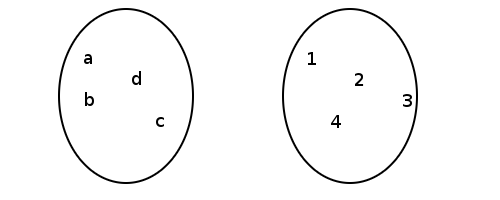
\includegraphics[width=250,height=700,
keepaspectratio]{imagens/conjuntos1.png}
\end{center}

\subsection{Extensão:}
Consiste em apresentar os elementos do conjunto listando-os.\\
\textbf{Exemplo 1.3:}\\ A = \{a,b,c,d\}\\ B = \{1,2,3,4,5\}\\ C = \{+,-,/,*\}\\

\subsection{Compreensão:}
Esta ´e a forma mais utilizada para representar conjuntos, consiste em descrever as regras que comp~oem a seleç~ao dos elementos que irao fazer parte de um conjunto. Escreve-se estas propriedades entre chaves descrevendo o termo geral(uma vari´avel qualquer) que denotara o elemento geral, e um barra separando-o das regras de produç~ao.

\textbf{Exemplo 1.4:} Utilizando-se dos conjuntos formados no exemplo 1.2, vamos representar os conjuntos A e B por compreensao;\\
A = $\{x \in \sum / x \geq a \wedge x \leq d\}$;\\
B = $\{x \in N / x \geq 1 \wedge x \leq 5\}.$\\ \\
\textbf{Obs:} No conjunto A, é possível conhecer os valores de cada letra do alfabeto através da Tabela ASCII (acrônimo para American Standard Code for Information Interchange) é uma codificação de caracteres de sete bits baseada no alfabeto inglês. Cada sequencia de códigos na tabela ASCII corresponde a um caractere.  Os códigos ASCII representam texto em computadores, equipamentos de comunicação, entre outros dispositivos que trabalham com texto. Desenvolvida a partir de 1960, grande parte das codificações de caracteres modernas a herdaram como base.

\section{Conjuntos Especiais:}
Na Teoria dos Conjuntos existem conjuntos ditos especiais, pois contem caracteristicas únicas que os diferenciam dos outros. Neste tópico apresentaremos estes conjuntos tal qual com sua definição e propriedades.
\subsection{Conjunto Vazio:}
O conjunto vazio é um conjunto no qual não contêm elementos, ou seja, sua cardinalidade é igual a 0. Este conjunto é representado por \{\} e principalmente por $\emptyset$.\\
\textbf{Exemplo 1.5:} Os exemplos de conjunto vazio são:\\ \\
A = $\{x \in IN / x \geq 0 \wedge x \leq -2 \}$\\
B = $\{x \in IN /  0 \div x \}$.
\\
\subsection{Conjunto Universo:}
Todos os elementos de um contexto alem de pertencerem aos seus respectivos conjuntos, eles também pertencem ao conjunto universo. Este é dito um conjunto especial pois varia de contexto para contexto, é denotado por $U$ é pode ser um conjunto inifinito ou finito. \\
\textbf{Exemplo 1.6:}\\ \\
A = \{x / x são todos os programas computáveis existem no mundo \};\\
U = \{x / x são todos os programas existem, sejam computáveis ou não \}.\\ \\

\subsection{Conjunto das Partes}
Chama-se Conjunto das Partes de um conjunto A, representado por P(A), todo conjunto formado por todos os subconjuntos de A. O total de subconjuntos do conjunto das partes é igual ao valor de $2^{n}$, sabendo que n é o número total de elementos pertencentes ao conjunto A.
\\
\textbf{Exemplo X.X:}\\
\begin{itemize}
\item C = $\{$a,b$\}$
\item P(C) = {$\emptyset$, $\{a\}$,$\{b\}$,$\{a,b\}\}$
\item[]
\item A = $\emptyset$
\item P(A) = $\{ \emptyset \}$ 
\end{itemize}

\section{Operações com Conjuntos}
\subsection{União de Conjuntos}
Dados dois conjuntos A e B, a união deles retrata em um conjunto C todos os elementos que pertencem a A conjuntamente a todos os elementos que pertencem a B. A união entre dois conjuntos é representado pelo símbolo $\cup$, então:\\
\begin{center}
$A \cup B$ = $\{x/ x \in A \vee x \in B \}$
\end{center}
A partir desta operação, podemos visualiza-la melhor através do seguinte diagrama de Venn.


\begin{center}
	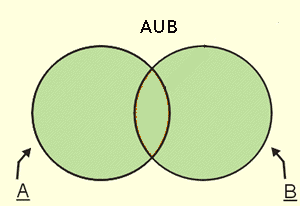
\includegraphics[scale=0.5]{imagens/unionConjuntos.png}
\end{center}

\\
\textbf{Exemplo 1.6:} Dados dois conjuntos A = $\{$a,e,i$\}$ e B = $\{$1,2,3$\}$, represente a união dois dois
\\
$A \cup B$ = $\{$a,e,i,1,2,3$\}$

\subsubsection{Propriedades da União}
\begin{enumerate}
\item $A \cup A = A$
\item $A \cup \emptyset = A$
\item $A \cup B = B \cup A$
\item $A \cup U = U$
\end{enumerate}
\subsection{Intersecção de Conjuntos}
Dados dois conjuntos A e B, a união deles retrata em um conjunto C todos os elementos que pertencem a A e também pertençam a B. A intersecção entre dois conjuntos é representado pelo símbolo $\cap$, então:\\
\begin{center}
$A \cap B$ = $\{x/ x \in A \wedge x \in B \}$
\end{center}
A partir desta operação, podemos visualiza-la melhor através do seguinte diagrama de Venn.

\begin{center}
	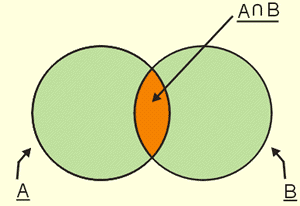
\includegraphics[scale=0.5]{imagens/IntersecConjuntos.png}
\end{center}
\\
\textbf{Exemplo X.X:} Dados dois conjuntos A = $\{$a,e,i$\}$ e B = $\{$1,2,3$\}$, represente a união dois dois:
\\
$A \cap B$ = $\emptyset$ , chamamos este caso particular de \textbf{conjuntos disjuntos}

\subsubsection{Propriedades da Intersecção}
\begin{enumerate}
\item $A \cap A = A$
\item $A \cap \emptyset = \emptyset$
\item $A \cap B = B \cup A$
\item $A \cap U = A$
\end{enumerate}
\subsection{Diferença de Conjuntos}
Sejam dois conjuntos A e B e sua diferença denotada por A - B. A diferença consiste em manter todos os elementos de A que não estão em B, ou seja, $\{ x/ x \in A \wedge x \ni B \}$.

\begin{center}
	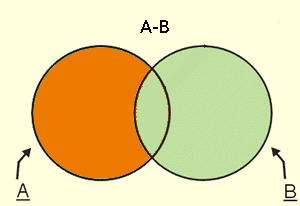
\includegraphics[scale=0.5]{imagens/diferencaConjuntos.png}
\end{center}
\\
\textbf{Exemplo X.X:} Dados dois conjuntos A = $\{$a,b,c,d,e$\}$ e B = $\{$a,e$\}$, resolva A - B:
\\
A - B = $\{$b,c,d$\}$\\


\subsubsection{Propriedades da Diferença}
\begin{enumerate}
\item $A - A = \emptyset$
\item $A - \emptyset = A$
\item $A - B \neq B - A$
\item $U - A = \bar{A}$
\end{enumerate}

\subsection{Complemento de um Conjunto}
Seja A um conjunto qualquer e U o conjunto universo, podemos retrar o complemento de através do símbolo $C_{A}^{U}$ ou $\bar{A}$. O complemento do conjunto A são todos os elementos que pertençam a U e que não pertençam ao conjunto A, isto indica uma diferença de U - A. Ou seja:
\\
\begin{center}
$\{x / x \in U \wedge x \ni A \}$
\end{center}

\begin{center}
	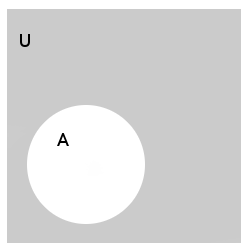
\includegraphics[scale=0.5]{imagens/complemento.png}
\end{center}

\\
\textbf{Exemplo X.X:} Seja o conjunto A = $\mathbb{N}$ e o U = $\mathbb{Z}$, então $\bar{A}$ será? $\mathbb{Z}$ - $\mathbb{N}$
\\

\subsubsection{Propriedades do Complemento}
\begin{enumerate}
\item $\bar{\bar{A}} = A$
\item $\bar{\emptyset} = U$
\item $\bar{U} = \emptyset$
\item $\bar{(A \cup U)} = \bar{A} \cap \bar{B}$
\item $\bar{(A \cap U)} = \bar{A} \cup \bar{B}$
\end{enumerate}
\subsection{União Disjunta}
No universo da teoria dos Conjuntos, existem operações classificadas em forma reversível e não reversível. No caso da união disjunta, é uma operação reversível da união normal. Uma operação reversível é retratada a partir do conjunto solução, ou seja, a partir do conjunto resposta é possível determinar os conjuntos originais que a comporam, coisa que na união normal seria impossível determinar. Uma união disjunta é denotada pelo símbolo $+$ e consiste em rotular com o conjunto origem, cada elemento que irá compor o conjunto solução.
 \\
\textbf{Exemplo X.X:}Dado o conjunto solução A + B = $\{1_{a},2_{a},2_{b},3_{b},4_{a},4_{b},5_{a},6_{a},7_{a},8_{a}, 8_{b}\}$\\
A = $\{$ 1,2,4,5,6,7,8$\}$\\
B = $\{$ 2,3,4$\}$
\\
\subsection{Produto Cartesiano}
O produto cartesiano é formado pelo par ordenado entre dois conjuntos A e B, onde todos os elementos são compostos com todos. A operação é denotada por A x B, onde $x \in A$ e $y \in B$, todos os pares ordenados serão formados da seguinte forma $(x,y)$.

\begin{center}
$\{(x,y) / x \in A \wedge y \in B \}$
\end{center}
 \\
\textbf{Exemplo X.X:}Seja dois conjuntos A = $\{$a,b,c$\}$ e B = $\{$a,e,i$\}$, apresente o produto cartesiano:\\
A x B = $\{$(a,a),(a,e),(a,i),(b,a),(b,e),(b,i),(c,a),(c,e),(c,i)$\}$\\

%%%%%%%%%%%%%%%%%%%%%%%%%%%%%%%%%%%%LOGICA%%%%%%%%%%%%%%%%%%%%%%%%%%%%%%%%%%%%%%%%%%%%%%%%
\chapter{Noções de Lógica}
Nas mais diversas áreas científicas a lógica tem sido cada vez mais presente, pela facilidade que ela trás para o desenvolvimento de provas. Lógica permite definir a noção de teorema. Em computação, um teorema freqüentemente pode ser visto como um problema a ser implementado computacionalmente, e sua correspondente demonstração, pode ser vista como uma
solução computacional, ou seja, um algoritmo. Adicionalmente, o algoritmo que
soluciona o problema, prova-se, sempre funciona.

\section{Proposição}
Uma proposição é uma sentença que pode adquirar o valor verdadeiro ou falso, geralmente denotador por letras minúsculas.
\\
\textbf{Exemplo 1.1:}
\\	  
\begin{itemize}
\item 10<7
\item Existe vida em outros planetas.
\item Todos os inteiros são pares.
\end{itemize}

\textbf{Nota}: O segundo exemplo é também uma proposição pois pode assumir o valor verdadeiro ou falso, por mais que não sejamos capazes de decidir qual dos dois.

\\
\textbf{Contra-Exemplo 1.1:} 
\\	  
\begin{itemize}
\item Como vai você?
\end{itemize}
O contra-exemplo é uma pergunta, não pode assumir valor-verdade, portanto não é um proposição.

\section{Conectivos Lógicos}
São símbolos que tornam possíveis a composição de proposições, afim de criar sentenças mais complexas. São com esses conectores que as tabelas verdades são construidas e analisadas.
\subsection{Conjunção}
Normalmente denotada pelo símbolo $\wedge$  (lê-se e). Se unirmos as duas proposições verdadeiras “Os elefantes são grandes” e “Bolas são redondas”, obteremos a proposição “Os elefantes são grandes e bolas são grandes” com o valor-verdade também verdadeiro.
Sendo p = “Os elefantes são grandes”  e  q = “Bolas são redondas” , temos que:
\begin{itemize}
\item Se \textbf{p} é verdadeiro e q é verdadeiro, então \textbf{p} $\wedge$ \textbf{q} (lê-se “p e q”) também será verdadeiro
\item Se \textbf{p} é verdadeiro e q é falso, então P $\wedge$ \textbf{q} será falso.
\item Se \textbf{p} é falso e q é verdadeiro, então P $\wedge$ \textbf{q} será falso.
\item Se \textbf{p} é falso e q é falso, então P $\wedge$ \textbf{q} é falso.
\end{itemize}

\begin{table}[htb]
\centering
\caption{Tabela verdade da conjunção}
     \sffamily \begin{tabularx}{1.0\textwidth}{ p{5cm}  p{5cm}  p{5cm} }
    \hline
   \textbf{p} \hfill & \textbf{q} \hfill & {$p \wedge q$} \\ \hline
    V & V & \textbf{V}\\
    V & F & \textbf{F}\\
    F & V & \textbf{F}\\
    F & F & \textbf{V}\\ \hline
    \end{tabularx} \normalfont
\label{table:Emissivity}
\end{table}

\\
\\
\textbf{Nota:} A conjunção só resultará em uma verdade quando as duas proposições forem também verdadeiras.
\\
\textbf{Exemplo 1.2:} 
\\	  
\begin{itemize}
\item Formigas são pequenas e bolas são quadradas.
\item “Formigas são pequenas” é verdadeiro e “bolas são quadradas” é falso. Portanto, “Formigas são pequenas e bolas são quadradas” é falso, pois só uma das proposições é verdadeira.
\end{itemize}

\subsection{Disjunção}
Normalmente denotada pelo símbolo ∨  (lê-se ou). Na disjunção de duas proposições, pelo menos uma das proposições terá de ser verdadeira(podendo as duas serem verdadeiras) para que a resultante seja uma verdade.
\begin{itemize}
\item Se \textbf{p} é verdadeiro e \textbf{q} é verdadeiro, então \textbf{p} $\vee$ \textbf{q} (lê-se “p ou q”) também será verdadeiro
\item Se \textbf{p} é verdadeiro e \textbf{q} é falso, então \textbf{p} $\vee$ \textbf{q} será verdadeiro.
\item Se \textbf{p} é falso e \textbf{q} é verdadeiro, então \textbf{p} $\vee$ \textbf{q} será verdadeiro.
\item Se \textbf{p} é falso e \textbf{q} é falso, então \textbf{p} $\vee$ \textbf{q} é falso.
\end{itemize}


\begin{table}[htb]
\centering
\caption{Tabela verdade da Disjunç~ao}
     \sffamily \begin{tabularx}{1.0\textwidth}{ p{5cm}  p{5cm}  p{5cm} }
    \hline
   \textbf{p} \hfill & \textbf{q} \hfill & {$p \vee q$} \\ \hline
    V & V & \textbf{V}\\
    V & F & \textbf{V}\\
    F & V & \textbf{V}\\
    F & F & \textbf{F}\\ \hline
    \end{tabularx} \normalfont
\label{table:Emissivity}
\end{table}
\textbf{Nota:} A disjunção só resultará em uma falsidade quando as duas proposições forem falsas.

\subsection{Negação}
Como dito anteriormente, uma proposição pode assumir o valor de falso ou verdadeiro. A negação de uma proposição é modificar o valor-verdade da mesma, introduzindo um não da forma mais apropriada. Comumente denotada por ¬p ou ~p.

\begin{itemize}
\item Se \textbf{p} = Brasil é um país,ent~ao ¬\textbf{p} = Brasil não é um país.
\item Se \textbf{p} é verdadeira, ¬\textbf{p} é falsa.
\item Se \textbf{p} é falsa,  ¬\textbf{p} é verdadeira.
\end{itemize}


\begin{table}[htb]
\centering
\caption{Tabela verdade da negaç~ao}
     \sffamily \begin{tabularx}{1.0\textwidth}{ p{5cm}  p{5cm}  }
    \hline
   \textbf{p} \hfill & ¬\textbf{p} \hfill  \\ \hline
    V & \textbf{F} \\
    F & \textbf{V} \\ \hline
    \end{tabularx} \normalfont
\label{table:Emissivity}
\end{table}


\subsection{Condição}
Denotada pelo símbolo $\rightarrow$ .A leitura da condição normalmente se dá por “Se...então...”. Na condição, temos que se partimos de uma premissa falsa, não temos como chegar em uma verdade. Por exemplo, se pensarmos na frase “Se eu acordar cedo amanhã, então vou encontrar um amigo.” Nossa premissa seria “Se eu acordar cedo amanhã”, se isso for verdadeiro, levando em consideração que a sentença “Se...então...” indica que se “...” acontecer, então “...” acontecerá, a conclusão não pode ser falsa. Caso ocorra, a proposição será falsa. (\textbf{p} $\rightarrow$ \textbf{q}, sendo \textbf{p} verdadeira e \textbf{q} falsa, será falso)

\begin{itemize}
\item Se \textbf{p} é verdadeiro e \textbf{q} é verdadeiro, então \textbf{p} $\rightarrow $ \textbf{q}(Lê-se “se P então \textbf{q}”) também é verdadeira.
\item Se \textbf{p} é verdadeiro e \textbf{q} é falso, então \textbf{p} $\rightarrow $ \textbf{q} será falsa.
\item Se \textbf{p} é falso e \textbf{q} é verdadeiro, então \textbf{p}$ \rightarrow $\textbf{q} será verdadeiro.
\item Se \textbf{p} é falso e \textbf{q} é falso, então \textbf{p}$ \rightarrow $\textbf{q} será verdadeiro. 
\end{itemize}


\begin{table}[htb]
\centering
\caption{Tabela verdade da condiç~ao}
     \sffamily \begin{tabularx}{1.0\textwidth}{ p{5cm}  p{5cm}  p{5cm} }
    \hline
   \textbf{p} \hfill & \textbf{q} \hfill & {$p \rightarrow q$} \\ \hline
    V & V & \textbf{V}\\
    V & F & \textbf{F}\\
    F & V & \textbf{V}\\
    F & F & \textbf{V}\\ \hline
    \end{tabularx} \normalfont
\label{table:Emissivity}
\end{table}


\subsection{Bicondição}
Denotada pelo símbolo $\leftrightarrow$. A bicondição reflete uma noção “nos dois sentidos”, ou seja, simultâneamente. Dado o conceito de condição, bicondição é a condição nos dois sentidos, na ida e na volta. A leitura da bicondição é “se e somente se”, o que especifíca a ideia de que um depende do outro.

\begin{itemize}
\item Se \textbf{p} é verdadeiro e \textbf{q} é verdadeiro, então \textbf{p} $\leftrightarrow$ \textbf{q} é verdadeiro. (Lê-se “\textbf{p} se e somente se \textbf{q}”)
\item Se \textbf{p} é verdadeiro e \textbf{q} é falso, então \textbf{p} $\leftrightarrow$ \textbf{q} é falso.
\item Se \textbf{p} é falso e \textbf{q} é verdadeiro, então \textbf{p} $\leftrightarrow$ \textbf{q} é falso.
\item Se \textbf{p} é falso e \textbf{q} é falso, então \textbf{p} $\leftrightarrow$ \textbf{q} é verdadeiro.
\end{itemize}

\begin{table}[htb]
\centering
\caption{Tabela verdade da bicondiç~ao}
     \sffamily \begin{tabularx}{1.0\textwidth}{ p{5cm}  p{5cm}  p{5cm} }
    \hline
   \textbf{p} \hfill & \textbf{q} \hfill & {$p \rightarrow q$} \\ \hline
    V & V & \textbf{V}\\
    V & F & \textbf{F}\\
    F & V & \textbf{F}\\
    F & F & \textbf{V}\\ \hline
    \end{tabularx} \normalfont
\label{table:Emissivity}
\end{table}

\section{Equivalências}
Dizemos que duas proposições são logicamente equivalentes (ou simplesmente equivalentes) quando os resultados de suas tabelas-verdade são idênticos. Uma conseqüência prática da equivalência lógica é que ao trocar uma dada proposição por qualquer outra que lhe seja equivalente, estamos apenas mudando a maneira de dizê-la. A equivalência lógica entre duas proposições, p e q, pode ser representada simbolicamente como: p  q, ou simplesmente por p = q.

\begin{center}
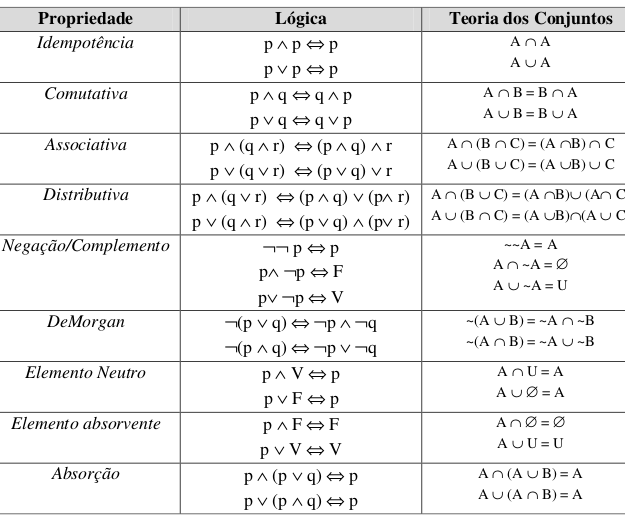
\includegraphics[scale=0.7]{imagens/tablePropriedades.png}
\end{center}

\section{Quantificadores}
Os quantificadores servem para transformar sentenças abertas em proposições lógicas, isto tudo sendo influenciado por uma váriavel.
\\
\textbf{Sentenças Abertas:}
\\
\begin{itemize}
\item x + 6 > 10;
\item x é um elefante.
\end{itemize}
Estas sentenças não denotam nada lógicamente, uma vez que não temos uma idéia de quantificação para a variável x, ou seja, não sabe-se seu intervalo de valores verdade.

\subsection{Quantificador Universal}
Quantificador universal, expande a variável para a idéia de "Para todo ...", comumente denotado por $\forall$ este quantificador é muito utilizado para se determinar a consideração de todos os elementos de um conjunto, tomamos como exemplo a expressão $x + 6 > 10$.\\ 
Não sabemos o que a variável $x$ esta representando e muito menos o quanto esta representando, porém ao utilizar o quantificar para a váriavel, podemos transcrever a função da seguinte forma, "Para todo x, tal que x + 6 é maior que 10" ou $\forallx, x + 6 > 10$.\\
Neste caso todos os valores possíveis para x terã que satisfazer a sentença. Neste caso a resposta seria falso, uma vez que se tomarmos os x = 2, a soma entre 2 + 6 não resultaria em um número acima de 10.


\subsection{Quantificador Existencial}
Este quantificador consiste em um caso mais restrito em relação ao quantificador universal, uma vez que o universal todos os elementos do conjunto domínio deveriam satisfazer a sentença, no caso do existencial se pelo menos um elemento satisfazer a sentença, então seu valor verdade é verdadeiro.\\
Então denotamos o quantificador existencial por $\exists$ e tomando como exemplo a sentença anterior temos $\exists x, x + 6 > 10$ e lê-se "Existe pelo menos um x, tal que x + 6 é maior que 10".Esta sentença é verdadeira.
%%%%%%%%%%%%%%%%%%%%%%%%%%%%END NOCOES DE LOGICA%%%%%%%%%%%%%%%%%%%%%%%%%%%%%%%%%%%%%%%

%%%%%%%%%%%%%%%%%%%%%%%%%%%%%%%%%%%%%%% OPERAÇ~OES ELEMENTARES %%%%%%%%%%%%%%%%%%%%%%%%%%%
\chapter{Operações Elementares}
Neste capítulo visa apresentar as operações elementares da matemática que servem de suma importância para o decorrer desta apostila. Todas as operações abordadas aqui são conhecidas por parte do leitor. Vamos trabalhar com potenciação e radiciação.

\section{Potênciação}
Calcular a potência de um número real equivale a multiplicar tal número n vezes. Observe  a baixo:
\\
\textbf{$a^{n}$}  = $\underbrace{a_{1} * a_{2} * a_{3} * … * a_{n}} $
\\
Na potenciação chamaos $a$ de base e $n$ de expoente. Sabendo que a potenciação consiste em uma forma simplificada de apresentar multiplicações por uma mesma base, vejamos as propriedades que as definem.

\subsubsection{Propriedades}
\begin{enumerate}
\item $a^{n} * a^{m} = a^{n + m}$
\item $\frac{a^{n}}{a^{m}} = a^{n - m}$
\item $a^{0} = 1$
\item $(a^{n})^{m} = a^{n * m}$
\item $a^{n^{m}} = a^{n_{1}*n_{2}*n_{3}*n_{4}*...*n_{m}}$
\item $(a * b)^{n}$
\item $(\frac{a}{b})^{n} = (\frac{a^{n}}{b^{n}})$, sendo b $\neq$ 0;
\item $a^{-n} = \frac{1}{a^{n}}$
\item $\sqrt[n]{a} = a^{\frac{1}{n}}, n > 0$;
\item $\sqrt[n]{a^{m}} = a^{\frac{m}{n}}, n > 0$;
\end{enumerate}

\subsection{Potenciação com expoentes Racionais}
Seja um número real, variável ou expressão algébrica e n um inteiro maior que 1. \\
\begin{center}
$a^\frac{1}{n} = \sqrt[n]{a}$
\end{center}
Se m é um inteiro positivo, $\frac{m}{n}$ está na forma reduzida e todas as raízes são números reais
\begin{center}
$a^\frac{m}{n} = (a^\frac{1}{n})^{m}$ e $a^\frac{m}{n} = (a^{m})^\frac{1}{n} = \sqrt[n]{a^{m}}$
\end{center}

\section{Raiz}
Seja n um número inteiro maior que 1 e a e b números reais.
Se $b^{n} = a$, então b é uma raiz n-ésima de a .
Se a tem uma raiz n-ésima, então a principal raiz n-ésima de a é aquela com o mesmo sinal de a .\\
A principal raiz n-ésima de a é denotada pela expressão com o radical $\sqrt[n]{a}$. O inteiro positivo n é o índice do radical e a é o radicando.
Se a é um número real positivo e n um número par positivo, suas duas raízes n-ésimas são denotadas por $\sqrt[n]{a}$ e -$\sqrt[n]{a}$.
\\
\textbf{Exemplo X.X}
\\
\begin{itemize}
\item $\sqrt[3]{\frac{28}{8}} = \frac{3}{2}$, porque $(\frac{3}{2})^{3} = \frac{27}{8}$
\end{itemize}
\\
\textbf{Exemplo X.X}
\\
\begin{itemize}
\item $\sqrt[4]{-625}$ , não é um número real porque o índice 4 é par e o radicando -625 é negativo (não existe número real cuja a quarta potência seja negativa).
\end{itemize}

\subsubsection{Propriedades}
\begin{enumerate}
\item $\sqrt[n]{ab} = \sqrt[n]{a} * \sqrt[n]{b}$
\item $\sqrt[n]{\frac{a}{b}} = \frac{\sqrt[n]{a}}{\sqrt[n]{b}}$
\item $\sqrt[m]{\sqrt[n]{a}} = \sqrt[n*m]{a}$
\item $(\sqrt[n]{a})^{n} = a$
\item $\sqrt[n]{a^{n}} = \pm a$
\end{enumerate}

\section{Racionalização}
Racionalizar é o processo de reescrever frações contendo radicais de modo que o denominador fique sem esses radicais. Quando o denominador tem a forma $\sqrt[n]{a^{m}}$, multiplicando numerador e denominador por $\sqrt[n]{a^{n - m}}$ poderemos eliminar o radical do denominador, porem existem três casos de eliminação que devemos considerar:

\subsubsection{Caso 1}
Neste caso o denominador é uma raiz quadrada, então basta multiplicar e dividir pela própria raiz que aparece no denominador:
\\
\textbf{Exemplo X.X}: Racionalize a seguinte expressão $\frac{\sqrt{y}}{y\sqrt{x}}$
\\
\begin{center}
$\frac{\sqrt{y}}{y\sqrt{x}}$\\ \\
$\frac{\sqrt{y}}{y\sqrt{x}}*\frac{\sqrt{x}}{\sqrt{x}}$\\ \\
$\frac{\sqrt{y}*\sqrt{x}}{y\sqrt{x^{2}}}$\\ \\
$\frac{\sqrt{yx}}{yx}$
\end{center}

\subsubsection{Caso 2}
O denominador é uma raiz ene-ésima, neste caso se no denominador há a raiz $\sqrt[n]{a^{m}}$, o fator a se racionalizar sera a raiz ene-ésima de um numero tal que complete uma potência de expoente n dentro do radical, ou seja, tomaremos $\sqrt[n]{a^{n-m}}$ como fator racionalizante. Com isto, simplificar a raiz ene-esima do denominador pelo expoente n resultante.
\\
\\
\textbf{Exemplo X.X}: Racionalize a seguinte expressão $\frac{2}{\sqrt[5]{9}}$
\\
Devemos lembrar que este caso, deve-se completar a potência do radicando afim de retira-lo da raiz. Então oberve que $\sqrt[5]{9} \Rightarrow \sqrt[5]{3^{2}}$. Para saber quanto precisa para completar basta fazer a seguinte operação $\sqrt[5]{3^{5 - 2}} = \sqrt[5]{3^{3}}$, sabendo disso temos:
\begin{center}
$\frac{2}{\sqrt[5]{9}}$\\ \\
$\frac{2}{\sqrt[5]{3^{2}}}$ \\ \\
$\frac{2}{\sqrt[5]{3^{2}}}*\frac{\sqrt[5]{3^{3}}}{\sqrt[5]{3^{3}}}$\\ \\
$\frac{2\sqrt[5]{3^{3}}}{\sqrt[5]{3^{2+3}}}$\\ \\
$\frac{2\sqrt[5]{27}}{3}$\\ \\
\end{center}

\subsubsection{Caso 3}
Neste caso o denominador é uma soma (diferença) envolvendo uma raiz quadrada. Deste modo, sendo o denominador por exemplo $a - \sqrt{b}$, temos que o fator racionalizante será $a + \sqrt{b}$, visto que ao multiplica-los aparecerá o produto da soma pela diferença de dois fatores, o que corresponde, pelo estudo dos produtos notáveis, a diferença de dois quadrados.
\\
\textbf{Exemplo X.X}: Racionalize a seguinte expressão $\frac{1}{3 - \sqrt{2}}$
\\
\begin{center}
$\frac{1}{3 - \sqrt{2}}$\\ \\
$\frac{1}{3 - \sqrt{2}} * \frac{3 + \sqrt{2}}{3 + \sqrt{2}}$ \\\\
$\frac{3 + \sqrt{2}}{3^{2} - \sqrt{2^{2}}}$\\ \\
$\frac{3 + \sqrt{2}}{9 - 2}$\\\\
$\frac{3 + \sqrt{2}}{7}$\\\\
\end{center}

%%%%%%%%%%%%%%%%%%%%%%%%%%%%%%%%%%%%%%%%%%%% FIM FUNÇOES ELEMENTARES %%%%%%%%%%%%%%%%%%%%%%%

%EXPRESSOES ALGEBRICAS%%%%%%%%%%%%%%%%%%%%%%%%%%%%%%%%%%%%%%%%%%%%%%%%%%
\chapter{Expressões Algébricas}
Uma expressão algébrica é toda expressão matemática na qual estão presentes letras ou símbolos que denotam grandezas genéricas que podem ser quaisquer valores no universo dos números. Essas expressões podem ser compostas sobre operações e sinais indicativos de prioridade. Note que essas letras são chamadas de incógnitas ou variáveis e são a parte príncipal das expressões algébricas.
\\
\textbf{Exemplo X.X:}
\begin{itemize}
\item $x^{2}$
\item $ \frac{x^{3}+4x}{2}$
\item $ 3y^{2}g^{3}$
\end{itemize}
\section{Monômio}
É uma expressão algébrica que não contêm operações de adição e nem subtração
\\
\textbf{Exemplo X.X:}
\begin{itemize}
\item $x^{2}$
\item $5x$
\item $ax^{2}$
\item $10$
\end{itemize}

\section{Binômio}
É a soma ou diferença de dois monômios.
\\
\textbf{Exemplo X.X:}
\begin{itemize}
\item $2x + y^{2}$
\item $3x - y$
\item $27h^{3}+ \frac{x + 2}{(x+2)^{2}}$
\end{itemize}


\section{Trinômio}
É a soma ou diferença de três monômios.
\\
\textbf{Exemplo X.X:}
\begin{itemize}
\item $2x^{2} - 5x + 10 + 20x = 2x^{2} + 10 + 15x$
\item $5x^{4} + 10x^{3} + x^{2}$
\end{itemize}


\section{Polinômio}
É a soma ou diferença de mais de três monômios.
\\
\textbf{Exemplo X.X:}
\begin{itemize}
\item $x^{5} + x^{4} + 3x^{3} = x^{4} + x^{3} + 3x^{2} $
\end{itemize}

\section{Produtos Notáveis}
Os produtos notáveis é uma maneira de apresentar uma determinada expressão de uma forma mais reduzida e de maior facílidade de entendimento. Apresentaremos neste etapa três produtos notáveis muito conhecidos e de grande importância para a matemática.

\subsection{Quadrado da soma de dois Termos}
O quadrado da soma de dois termos esta associado a potenciação. Visto que 10.10 = 10^{2}, então pode-se dizer que $x.x =  x^{2}$. Porem o que seria o quadrado de dois termos? Digamos que temos dois valores x e y, e que precisamos do quadrado da soma desses números, para qualquer $x,e \in \Re$. Temos então a seguinte expressão:
\\
 
\begin{center}
 $(x + y)^{2} = (x + y).(x + y)$
\end{center} 
\\
Agora visualizando pode se ver a quadrado da soma. Então que deve ser feito é uma distributiva dos elementos do primeiro termo, com os do segundo, afim de manter a coerência da conta, então:
\\
\begin{center}
$(x + y).(x + y) \Rightarrow x(x + y) + y(x + y) \Rightarrow x^{2} + xy + yx + y^{2} \Rightarrow x^{2} + 2xy + y^{2}$
\end{center}
\\
Portanto, $\forall x,y \in \Re$  :
\\
$(x + y)^{2} = x^{2} + 2xy + y^{2}$


\subsection{Quadrado da diferença de dois Termos}
Vamos utilizar o mesmo principio abordado da subseção anterior, porem agora estaremos trabalhando com a diferença das variáveis x e y: 
\begin{center}
$(x - y)^{2} = (x - y).(x - y)$ 
\end{center}
\\
Agora visualizando pode se ver a quadrado da diferença. Entao que deve ser feito e uma distributiva dos elementos do primeiro termo, com os do segundo, afim de manter a coêrencia do cálculo, entao:
\\
\begin{center}
$(x - y).(x - y) \Rightarrow x(x + y) + y(x + y) \Rightarrow x^{2} - xy - yx + y^{2} \Rightarrow x^{2} - 2xy + y^{2}$
\end{center}
\\
Portanto, $\forall x,y \in \Re$  :
\\
\begin{center}
$(x - y)^{2} = x^{2} - 2xy + y^{2}$
\end{center} 
\\
Então, mesmo sendo duas operações diferentes soma e subtração, a única diferença entre o quadrado da soma e da diferença é o sinal da composição dos termos diferentes de ambas as expressões.
\subsection{Produto da Soma pela diferença}
Tambem conhecido como diferença de dois quadrados e o produto de duas expressões da forma (x + y)(x - y). Para realizar está equação devemos multiplicar o primeiro fator pelo segundo. Segue abaixo a demonstração
\\
\begin{center}
$(x + y)(x - y) \Rightarrow x(x - y) + y(x - y) \Rightarrow x^{2} - xy + yx - y^{2} \Rightarrow x^{2} - y^{2}$
\end{center}
\\
Portanto, podemos concluir que:
\\
\begin{center}
$(x + y)(x - y) \Rightarrow x^{2} - y^{2}$
\end{center}

\section{Fatoração}
A partir dos produtos notaveis estudados, podemos introduzir o assunto de fatoração. A fatoração é extremamente importante para se poder aplicar as propriedades matemáticas afim de simplificar as expressões, uma forma de fatoração muito destacada são as frações, quando adequamos tanto o numerador quanto o denominador para podermos chegar sempre na forma mais simplificada da expressão. Uma fatoração consiste em dado uma expressão algébrica, evidênciar seus elementos em comum mediante a propriedades distributiva. 
\\
\\
\subsection{Evidência}
\textbf{Exemplo X.1:}
\\
Seja uma expressão algébrica $30x^{2}y^{3} + 5xy^{2}$, podemos notar que dentro desta expressão existem 3 elementos diferentes um do outro, porém estão em comum dentre os dois fatores são o número 5, a variável x e a variável $y^{2}$. Visto os elementos destacados chamamos de \textbf{fator comum} e o próximo passo será coloca-los em evidência $5xy^{2}(6xy + 1)$. No fim a expressão obtida, pode ser transformada na original através da propriedades distributiva.\\
\\
\subsection{Fatoracao por Agrupamento}
\textbf{Exemplo X.12:}
\\
Seja uma expressão algébrica $x^{3} - 2x^{2}y + xy - 2y^{2}$, é importante notar que a disposição dos elementos da expressão não importa, desde que a estrutura aritmética não seja alterada. Neste caso utilizaremos um método chamado \textbf{fatoração por agrupamento}, que consiste em rearanjar os elementos afim de manter os elementos a serem fatoras juntos. Então a partir da expressão dada, tem-se um reagrupamento:
\\
\begin{center}
$[x^{3} - 2x^{2}y] + [xy^{2} - 2y^{3} ]$ 
\end{center}
\\	
No primeiro colchetes, a variável em comum dentre os dois termos é $x$ com o expoente na 2, então o fator comum entre as duas consiste em $x^{2}$; no segundo colchete é fácil notar que o único elemento em comum é a variável $y$ e que seu expoente é 2. Então temos que $y$ é o fator comum dentre os dois termos:
\\
\begin{center}
$x^{2}(x - 2y) + y^{2}(x - 2y)$ 
\end{center}
\\
Porem esta expressão pode ser fatorada ainda mais, uma vez que existem dois termos com coeficientes em comum, mas esse fator comum consiste na expressão algébrica $(x - 2y)$. Então pelas propriedades da fatoração, temos a seguinte expressão fatorada:
\\
\begin{center}
$(x^{2} + y^{2}).(x - 2y)$
\end{center}
\\
\subsection{Fatoraçao por produtos notaveis}
\textbf{Exemplo X.12:}
\begin{itemize}
\item $x^{2}$
\item $x^{2} - 2xy + y^{2}$
\item $x^{2} - y^{2}$
\end{itemize}
Note que todas essas expressões acima ja são conhecidas, estas foram apresentadas na seção de produtos notáveis. Produtos notaveis são nada mais nada menos que expressões algébricas fatoradas a uma forma miníma, as que foram apresentadas e trabalhadas sao as mais utilizadas e aplicadas. Vejamos então algumas derivações destas
\begin{itemize}
\item Dada a expressão $4x^{2} - 4xy + y^{2}$ fatore a para sua forma minima:
\\
Quando visuzalizamos uma expressão desta forma, logo podemos recorrer ao quadrado da diferença de dois termos. Uma vez que se formos fatorar pelo modo convencional, nunca chegaremos a forma mais fatorada da expressão que é:
\\
\begin{center}
$4x^{2} - 4xy + y^{2} = (2x^{2} - y^{2})^{2}$
\end{center}
\item Dada a expressão $x^{2} + 8x + 16$ fatore a para sua forma miníma:
\\
Note que a expressão dada é exatamente a mesma do exemplo anterior, com algumas modificações quanto aos dois termos. Uma forma de identificar quais são os termos envolvidos no expressão é quebrando a expressão o máximo que for possível, então: 
\\
\begin{center}
$x.x + 2.(4x) + 4.4$
\end{center}
Desta forma fica mais fácil identificar cada um dos termos, vamos utilizar a fórmula obtida pelo quadrado da soma de dois termos, $x^{2} + 2xy + y^{2}$ pode se ver que a constante 2 esta multiplicando o produto do primeiro termo pelo segundo, e o restante da equaçao é básicamente os termos elevados ao quadrado. Assim podemos inferir que o primeiro termos e a variavel $x$ e o segundo seria a constante 4. Deste modo, utilizando as propriedades do quadrado da soma de dois termos, temos.
\\
\begin{center}
$(x + 4)^{2}$
\end{center}
\\
\end{itemize}
\subsection{Trinomio de segundo grau}
Chama-se desta maneira pois estão envolvidos 3 termos e o termo de maior grau esta elevado ao quadrado. Esta forma de fatoraçao e um pouco mais trabalhosa de se resolver, uma vez que não existe um produto notável que simplifique esta compreensão. Vejamos melhor com um exemplo:
\\
\textbf{Exemplo X.X:} Seja a expressão $x^{2} - 5x + 6$
\\
Pode-se resolver essa fatoração utilizando a fórmula de Bhaskara:
\\
\begin{center}
$\frac{-b \pm \sqrt[2]{b^{2} - 4ac}}{2.a}$
\end{center}
\\Utilizando esta fórmula teremos como resposta dois valores o x' e x'', chamadas raízes da equação. Estas raízes serão colocadas pela definição da seguinte forma:\\
\begin{center}
$a(x - x').(x - x'')$
\end{center}
\\
Então a partir de uma pequena definição, podemos prosseguir com a resolução do exemplo utilizando a regra da bhaskara. Primeiramente devemos definir nossos parâmetros a,b e c. Seja  $a = 1$, $b = -5$ e $c = 6$, temos a seguinte construção da fórmula.
\\
\begin{center}
$\frac{-(-5) \pm \sqrt[2]{5^{2} - 4.1.6}}{2.1}$
\\
$\frac{5 \pm \sqrt[2]{25 - 24}}{2}$
\\
$\frac{5 \pm 1}{2}$
\\
$x' = \frac{5 + 1}{2} \Rightarrow \frac{6}{2} \Rightarrow x' = 3$
\\
$x'' = \frac{5 - 1}{2} \Rightarrow \frac{4}{2} \Rightarrow x'' = 2$
\end{center}
Temos então como respostas da equação de bhaskara que é x' = 3 e x'' = 2, então a fatoração final ficará:
\\
\begin{center}
$(x - 3).(x - 2) \Rightarrow x^{2} -5x +6$
\end{center}
Note que a forma de fatoração desta expressão é bem mais facilitada pela utilização de uma fórmula de Bhaskara.
\section{Simplificação de Frações Algébricas}
Uma das principais necessidades é a fatoração ou simplificação das expressões algébricas dentro de frações. As frações algébricas dependendo das expressões em que nelas estão envolvidas, podem se tornar complicas de se entender na sua forma pura, então é necessário uma simplificação afim de minimiza-las e torna-las mas operáveis. Primeiramente vamos relembrar as partes de uma fração e depois iremos abordar as simplificações que podem ser feitas.
\\
Uma fração é divida em duas partes o numerador e o denominador:
\\
\begin{center}
$\frac{numerador}{denominador}$
\end{center}
\\
O numerador consiste na parte inteira e o denominador significa o número de frações em que a parte inteira será submetida a divisão. Porém uma fração não so é constituida de números, quando a presença de expressões chamamos esta situação de expressões algébricas.
\\
\textbf{Exemplo X.12:}
\\
\begin{itemize}
\item $\frac{y}{x}$
\item $\frac{2x^{2} + y}{x + y}$
\end{itemize}
Do mesmo modo ao efetuarmos uma simplificação de frações numéricas, é possível realizar a simplificação de frações algébricas, utilizando o metodo da fatoração ou Briot-Ruffini.

\subsection{Simplificação com Fatoração}
Utilizando dos métodos de fatoração aprendidos da seção X.X, vamos realizar algumas simplificações de frações. Note que sempre que haver termos iguais tanto no numerador quanto no denominador, podemos anula-los. Veremos agora alguns exemplos para melhor entender o assunto.
\\
\textbf{Exemplo X.12:} Seja a fração $\frac{4x^{2} +16x + 16}{4x^{2} + 8}$ realize a simplificação: 
\\
Primeiramente nota-se que o numerador contem uma expressão ja conhecida. Caso não tenha ficado evidente, vamos organiza-la para uma melhor visualização.
\\
\begin{center}
$ \frac{2x.2x + 2.4.2x + 4.4}{4x^{2} + 8}$
\end{center}
\\
Percebeu? No numerador temos o quadrado da soma de dois termos, um produto notável. Ja sabemos a sua forma simplificada a partir da regra do quadrado, então vamos simplifica-lo.
\\
\begin{center}
$ \frac{(2x + 4)^{2}}{4x + 8}$
\end{center}
\\
Bom temos a simplficação completa do numerador, porem ainda é necessario realizar a simplificação do denominador. Utilizando o número 2 como fator comum, teremos a seguinte expressão.
\\
\begin{center}
$ \frac{(2x + 4)^{2}}{2(2x + 4)} \Rightarrow \frac{(2x + 4)}{2}$
\end{center}
\\
A partir do fator comum 2 do denominador, foi possível igualar ambas as expressões das partes envolvidas na fração e por fim realizar a simplificação. Deixando somente a parte restante do numerador, lembrando que o numerador era o dobro do denominador.
\\
\textbf{Exemplo X.X:} Seja a fração $\frac{x^{3}y - 2x^{2}y^{2}}{x^{2} - 4xy + 4y^{2}}$ realize a simplificação: 
\\
Primeiramente vamos fatorar o numerador, visando sempre evidenciar o fator comum. Teremos então:
\\
\begin{center}
$\frac{x^{3}y - 2x^{2}y^{2}}{x^{2} - 4xy + 4y^{2}} \Rightarrow \frac{x^{2}y(x - 2y)}{x^{2} - 4xy + 4y^{2}}$
\end{center}
\\
Ja o denominador é um produto notável, o quadrado da diferença de dois termos. Então escrevemos:
\\
\begin{center}
$x^{2} - 4xy + 4y^{2} \Rightarrow (x - 2y)^{2}$
\end{center}
\\
No fim teremos a seguinte expressão:
\\
\begin{center}
$\frac{x^{3}y - 2x^{2}y^{2}}{x^{2} - 4xy + 4y^{2}} \Rightarrow \frac{x^{2}y(x - 2y)}{(x - 2y)^{2}} \Rightarrow \frac{x^{2}y(x - 2y)}{(x - 2y).(x - 2y)} \Rightarrow \frac{x^{2}y}{x - 2y}$
\end{center}
\\
\subsection{Briot-Ruffini}
O método de simplificação de polinômios de Briot-Ruffini, foi criado por Paolo Ruffini. Este algorítmo consiste em uma simplificação de expressão algébrica, utiliza-se os coeficientes desse polinômio afim de reduzir o grau da equação toda. O Briot-Ruffini pode ser aplicado a qualquer polinômio que satisfaça as seguintes propriedades:
\\
\begin{itemize}
\item $\exists a \in \Re $ desenvolva a expressão ao valor 0.
\item Caso este o item acima é verificado, é realizado o algoritmo de Briot-Ruffini e o seu resultado será multiplicado pelo binômio $(x - a)$.  
\end{itemize} 
\\
Vejamos um exemplo para firmar os conceitos abordados.
\\
\\
\textbf{Exemplo X.X:} 
\\
Seja o binômio $x^{2} - x$ utilize o método de Briot-Ruffini para simplificar a expressão: 
\\
\begin{itemize}
\item Primeiramente observando a regra abaixo, acharemos um valor qualquer para x, que zere a função.
\item Tendo este valor, desenhe uma tabela como na figura X.X para colocando o x na primeira coluna e na segunda linha. E os coeficientes de maior grau da esquerda para a direita na primeira linha e segunda coluna
\item Por fim o coeficiente de maior grau e mantido, e partir deste ponto sera multiplicado o valor de x pelo grau atual e somado com o (grau - 1).
\end{itemize}

\begin{center}
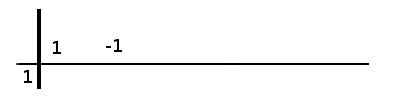
\includegraphics[scale=0.7]{imagens/briotRuffini.png}
\end{center}
\\
No fim aplicando o algoritmo de Ruffini, obteremos a equacao simplificada:
\\
\begin{center}
$x^{2} - x \Rightarrow (x - 1)x$
\end{center}
%%%%%%%%%%%%%%%%%%%%%%%%%%%%%%%%%%%%%%%%% END EXPRESSOES ALGEBRICAS %%%%%%%%%%%%%%%%%%%%%%%%%%%%%%%%%%%%



%%%%%%%%%%%%%%%%%%%%%%%%%%%%%%%%%%%%%%%%%%INEQUACOES%%%%%%%%%%%%%%%%%%%%%%%%%%%%%%%%%%%%%%%%%%%%%%%%%%%%%%%
\chapter{Inequações}
Inequação é uma sentença matemática expressadas por uma desigualdade, diferenciando da equação que representa uma igualdade. Essas sentenças contêm duas ou mais incógnitas, que serão utilizadas para montar os intervalos.
Porém antes de adentrarmos no assunto de inequações, vamos relembrar algumas desigualdades e suas propriedades:
\subsection{Desigualdades}
Para podermos dizer que um número real é maior ou menor que outro, devemos introduzir o conceito de numero real positivo e uma relação de ordem.
\\
\subsubsection{Axioma de Ordem}
No conjunto dos numeros reais existe um subconjunto denominado de números positivos, tal que:
\begin{enumerate}
\item Se $a \in \Re$, exatamente uma das três afirmações ocorre: a= 0; a é positivo; -a é positivo
\item A soma de dois números positivos é positiva;
\item O produto de dois números positivos é positivo;
\item Um n´umero real $a$ é negativo se e somente se -a é positivo.
\end{enumerate}
\subsubsection{Símbolos}
Para expressarmos estas relações de ordem, utilizamos alguns símbolos que facilitem a interpretação do problema. Apesar dessa interpretação ser facilitada aos ser observada com números, porem na presença de expressões algébricas ela se torna mais complicada.
\\
\begin{itemize}
\item Os símbolos $<$ (menor que) e $>$ (maior que) são defínidos:
	\begin{enumerate}
	\item $a < b \Leftrightarrow b - a$ é positivo;
	\item $a > b \Leftrightarrow a - b$ é positivo; 
	\end{enumerate}
\item Os símbolos $\leq$ (menor ou igual que) e $\geq$ (maior ou igual que) são definidos:
	\begin{enumerate}
	\item $a \leq b \Leftrightarrow a < b ou a = b$;
	\item $a \geq b \Leftrightarrow a > b ou a = b$;
	\end{enumerate}
\end{itemize}
As expressões envolvendo os símbolos acima são chamadas de \textbf{desigualdades}. $a < b$ e $a > b$ são desigualdades estritas enquando $a \leq b$ e $a \geq b$ são desigualdades não estritas.

\subsubsection{Propriedades}
Sejam $a,b,c,d \in \Re$ 
\begin{enumerate}
\item Se $a > b$ e $b > c$, então $a > c$;
\item Se $a > b$ e $c > 0$, então $ac > bc$;
\item Se $a > b$ e $c < 0$, então $ac < bc$;
\item Se $a > b$, então $a + c > b + c \forall c \in \Re$;
\item Se $a > b$ e $c > d$, então $a + c > b + d$;
\item Se $a > b > 0$ e $c > d > 0$, então $ac > db$.
\end{enumerate}
Todas as propriedades acima verificam a veracidade das operações das desigualdades. Utilizando as propriedades de lógica pode facilmente identifica-las entre as propriedades, como por exemplo a transitividade na propriedade 1.

\subsection{Valor Absoluto}
Também chamado de módulo de uma expressão é a distância que um determinado ponto se encontra até a origem ( ponto de intersecção entre o eixo das abscissas e das ordenadas). O módulo de qualquer número é ele mesmo so que positivo, pois a distância entre quaisquer pontos nunca pode ser negativa.

\subsubsection{Definição}
O valor absoluto de $a$, denotado por $|a|$, e definido como:
\\
$|a| = a$, se $a \leq 0$.\\
$|a| = -a$, se $a < 0$.
\\
\\
\subsubsection{Interpretação Geométrica}
Geometricamente o valor absoluto de a, também chamado de módulo de a, representa a distância de $a$ e 0. Escreve-se então $|a| = \sqrt{a^{2}} \Rightarrow \pm a$
\subsubsection{Propriedades}
\begin{enumerate}
\item $|x| < a \Leftrightarrow -a < x < a$, onde $a > 0$;
\item $|x| > a \Leftrightarrow x > a$ ou $x < -a$, onde $a > 0$;
\item Se $a,b \in \Re$ e $b \neq 0$, então $|\frac{a}{b} = \frac{|a|}{|b|}$;
\item Se $a,b \in \Re$, então $|a \pm b| \leq |a| + |b|$;
\item Se $a,b \in \Re$, então $|a| - |b| \leq |a - b|$.
\end{enumerate}

\section{Inequações de Primeiro grau}
Chama-se inequação de 1º grau, na variável x, a qualquer expressão algébrica que possa ser reduzida a uma das formas:
\\
Sabendo que $a,b \in \Re e a \neq 0$:
\begin{enumerate}
\item $ab + b < 0$;
\item $ab + b \leq 0$;
\item $ab + b > 0$;
\item $ab + b \geq 0$;
\end{enumerate}
O resultado de uma inequação não consiste em um único valor real e sim em um conjunto de valores que tornem a desigualdade verdadeira. Para obtermos o conjunto solução de uma inequação do primeiro grau, podemos utilizar o processo dedutivo, que consiste em isolar a variável x, realizando, para isto, operações inversas na ordem inversa. Devemos notar também que toda vez que há necessidade de multiplicar ou dividir a inequação intera por $(-1)$, deve se inverter o símbolo de desigualdade.
\\
\\
\textbf{Exemplo X.X:} Seja a inequação $-3x \leq 6$, encontre o conjunto solução: 
\\
\begin{itemize}
	\item $3x \leq -6 \rightarrow$ Multiplicação por (-1), inverte o sinal da desigualdade;\\
	\item $x \geq \frac{-6}{3} \rightarrow$ Isolar o x;\\
	\item $x \geq -2 \rightarrow$ A veracidade da inequação somente para valor para x maiores ou iguais a -2.\\
	
\end{itemize}
O resultado pode ser expresso em intervalo $[-2 ; +\\infty)$. As respostas são geralmente escritas na forma de intervalos, pois torna mais abstrato e mais compacto representar o conjunto solução
\\
\textbf{Exemplo X.X:} Seja a inequação $\frac{x}{3} + \frac{1}{2} > \frac{x}{4} + \frac{1}{3}$, encontre o conjunto solução: 
\\
\begin{itemize}
	\item $\frac{2x + 3}{6} > \frac{3x + 4}{12} \rightarrow$ Descobrir o mmc de ambos os lados
	\item $12(2x + 3) > 6(3x + 4) \rightarrow$ Multiplica ambos os denominadores dos dois lados
	\item $24x + 36 > 18x + 24 \rightarrow$ Aplicando a distributividade temos a seguinte expressão
	\item $24x - 18x > -36 + 24 \rightarrow$ Isolar o x
	\item $6x > -12$
	\item $x > -2$	
\end{itemize}
O conjunto solução é o intervalo $(-2 ; +\infty)$, vale ressaltar que diferentemente do exemplo X.X o exemplo X.X apresenta um intervalo aberto, pois não engloba o elemento -2. Então para x = -2 a desigualdade não será verdadeira.
\\
\\
\textbf{Exemplo X.X:} Seja a inequação $ -3 < \frac{2x + 5}{3} \leq 5 $, encontre o conjunto solução: 
\\
\begin{itemize}
	\item $ -3.3 < \frac{3.(2x + 5)}{3} \leq 5.3  \rightarrow$ Multiplicar todas as partes da inequação por 3
	\item $ -9 -5 < 2x + 5 -5 \leq 15 -5 \rightarrow$ Soma em todas as partes da inequação o valor -5.
	\item $ \frac{-14}{2} < \frac{2x}{2} \leq \frac{10}{2} \rightarrow$ Divide todas as partes da inequação por 2
	\item $ -7 < x \leq 5 \rightarrow$ Como o x ja esta isolado, então ja tem-se o conjunto solução
\end{itemize}
Também representado pela notação de intervalo como $(-7;5]$, note que nesta inequação resolvemos as inequações envolvias simultâneamente, porém também é possível dividir a inequação em duas e resolver uma de cada vez
\\
\\
\textbf{Exemplo X.X:} Seja a inequação $ 1 \leq 2x + 3 < x + 5 $, encontre o conjunto solução: 
\\
Primeiramente, note que existem duas inequações de primeiro grau nesta sentença, a primeira consiste em $1 \leq 2x + 3$ e a segunda inequação é $2x + 3 < x + 5$. Então vamos resolve-las separadamente:
\subsubsection{Primeira Inequação: 1 \leq 2x + 3}
\begin{itemize}
\item  $1 - 3 \leq 2x \rightarrow$ Isolar o x
\item  $ \frac{-2}{2} \leq x$ 
\item  $ -1 \leq x$
\end{itemize}
Temos na primeira parte da inequação que $x \leq -1$, porem antes de montar o conjunto solução precisamos resolver a segunda parte da inequação.
\subsubsection{Segunda Inequação: 2x + 3 < x + 5}
\begin{itemize}
\item  $2x + 3 < x + 5 \rightarrow$ Isolar o x
\item  $ 2x - x < 5 - 3$ 
\item  $ x < 2$
\end{itemize}
Agora podemos fechar nosso conjunto solução, vamos analisar os resultados $x \leq -1$ e $x < 2$. Nesta parte para conseguir fecharmos o conjunto solução o x tem que satisfazer as duas soluçoes simultâneamente. Isto nos da alusão de uma conjunção lógica em que $\{x \in \Re / x \geq -1 \wedge x < 2\}$.\\
Visto que o x satisfaz ambas as soluções, então temos o intervalo solução $[-1;2)$

\section{Inequações de Segundo grau}
Define-se grau de uma inequação a partir do maior expoente entre todas as incógnitas, se $\forall a,b,c \in \Re$ e $a \neq 0$  temos:
\begin{itemize}
\item $ax^{2} + bx + c > 0$
\item $ax^{2} + bx + c < 0$
\item $ax^{2} + bx + c \leq 0$
\item $ax^{2} + bx + c \geq 0$
\end{itemize}
Todas as inequações acima são denominadas de 2º Grau. A forma para resolve-la é análoga a resolução de funções de 2º grau, através do método de Bhaskara. Porém antes de abordarmos essa forma novamente, vamos realizar um estudo dos gráficos e como seus grandezas alteram-se. Esta observação é subdividida em dois casos:
\subsubsection{Caso 1}
Se $a > 0$ teremos uma parábola com sua concavidade voltada para cima, conforme apresenta a figura abaixo:\\
\begin{center}
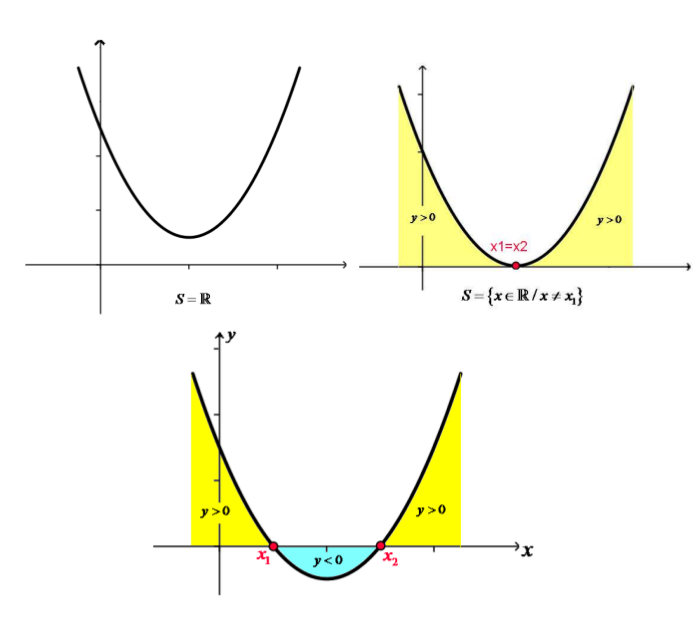
\includegraphics[scale=0.5]{imagens/grafGrau2Case1.png}
\end{center}

E também a partir do $\Delta$ teremos a posição da parábola no gráfico então temos as seguintes situações:
\begin{itemize}
\item Se $\Delta > 0$ tem-se o seguinte gráfico:\\
	\begin{center}
	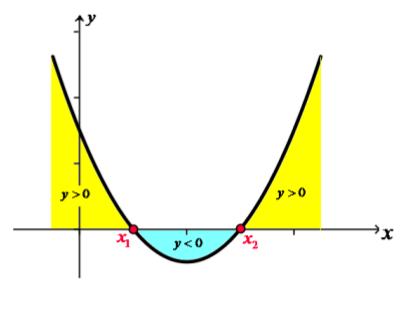
\includegraphics[scale=0.5]{imagens/deltaGrau2Grafi.png}
	\end{center}
\item Se  $\Delta = 0$ desenvolve-se o seguinte gráfico:\\
	\begin{center}
	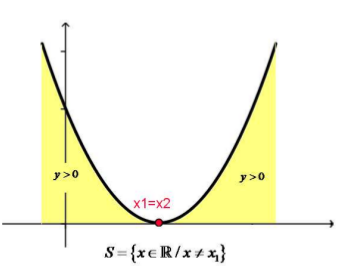
\includegraphics[scale=0.5]{imagens/deltaGrau02Grafi.png}
	\end{center}
\item Se $\Delta < 0$ a função quadrática não admite zeros reais. A parábola não intercepta o eixo:\\
	\begin{center}
	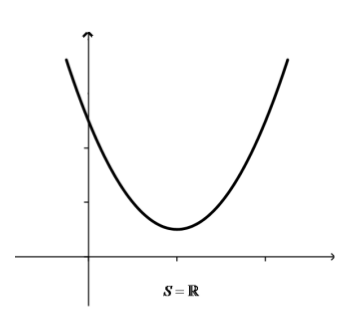
\includegraphics[scale=0.5]{imagens/grafCase1DeltaMe0.png}
	\end{center}
\end{itemize}

\subsubsection{Caso 2}
Se $a < 0$ teremos uma parábola com sua concavidade voltada para baixo, conforme apresenta a figura abaixo:\\
\begin{center}
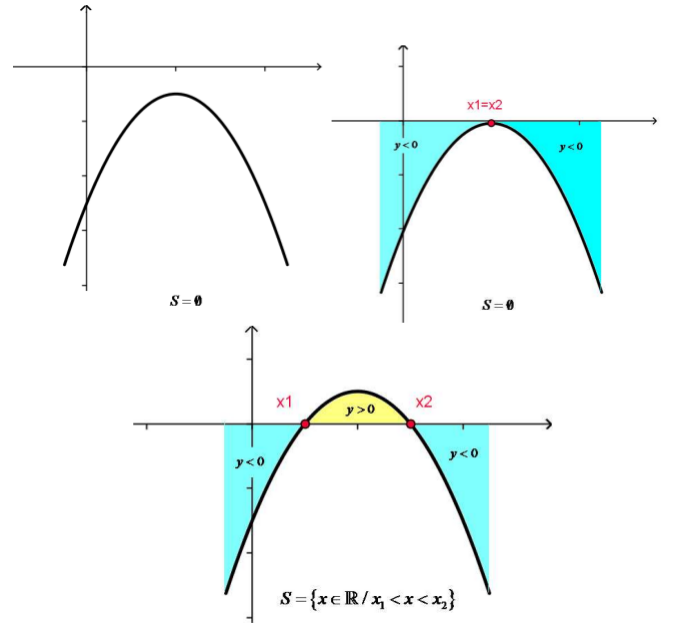
\includegraphics[scale=0.5]{imagens/grafGrau2Case2.png}
\end{center}

Assim como no caso 1, vamos apresentar como ficara as posições do gráfico em função de $\Delta$
\begin{itemize}
\item Se $\Delta > 0$ tem-se o seguinte gráfico:\\
	\begin{center}
	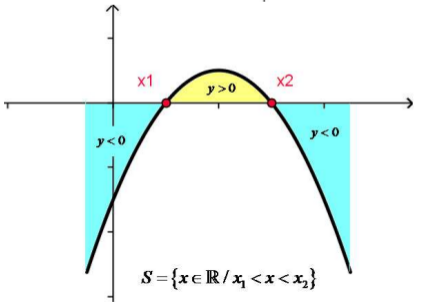
\includegraphics[scale=0.5]{imagens/deltaGrau22Grafi.png}
	\end{center}
	\\
\item Se  $\Delta = 0$ desenvolve-se o seguinte gráfico:\\
	\begin{center}
	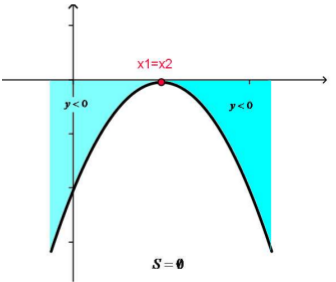
\includegraphics[scale=0.5]{imagens/deltaGrau202Grafi.png}
	\end{center}
\item Se $\Delta < 0$ a função quadrática não admite zeros reais. A parábola não intercepta o eixo:\\
	\begin{center}
	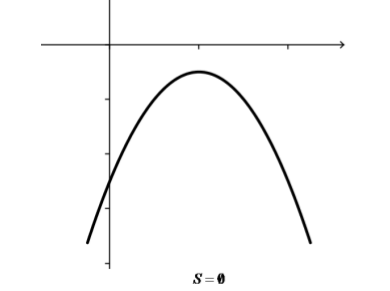
\includegraphics[scale=0.5]{imagens/grafCase21DeltaMe0.png}
	\end{center}
\end{itemize}

\subsubsection{Resolução}
A resoluç~ao de uma inequação de segundo grau pode ser resumida em três etapas:
\begin{itemize}
\item Resolver a equação de segundo grau utilizando a fórmula de Bhaskara $\frac{-b \pm \sqrt{b^{2} - 4ac}}{2.a}$;
\item Estabelecer a variação de sinais do trinômio $ax^{2} + bx + c$, segundo as seguintes regras:
	\begin{enumerate}
		\item Se a equação admite duas raízes, ou seja, $\Delta > 0$, então a regra a ser seguida é:	
		\begin{flushleft}
		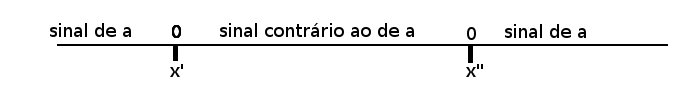
\includegraphics[scale=0.53]{imagens/resolucaoIneGrau2.png}
		\end{flushleft}
		
		\item Se a equação admite dua raízes iguais $x'$ e $x''$ a regra a ser seguida é:
		\begin{flushleft}
		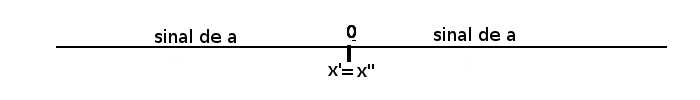
\includegraphics[scale=0.53]{imagens/resolucaoIneGrau22.png}
		\end{flushleft}
		
		\item Se a equação não admite raízes reais, a regra a ser seguida é: \textbf{O sinal da inequação é o mesmo de $a$}
	\end{enumerate}
\item Apresentar a solução algébrica, atendendo as desigualdades fixadas pela inequação. A forma mais explorada a ser usado é a de intervalos.
	
\end{itemize}
\\
\textbf{Exemplo X.X:} Seja a inequação $x^{2} - x - 12 > 0$, encontre o conjunto solução: 
\\	
\begin{itemize}
\item Primeiramente devemos resolver a equação de segundo grau afim de encontrar as raízes x' e x'';
\begin{center}
Sabendo que $a = 1$,$b = -1$ e $c = -12$, utilizando-os na fórmula de Bhaskara temos:\\
$\frac{-(-1) \pm \sqrt{(-1)^{2} 4.1.(-12)}}{2.1} \Rightarrow$
\end{center}
\\
\begin{center}
$\frac{1 \pm \sqrt{49}}{2} \Rightarrow$
\end{center}
\\
\begin{center}
$\frac{1 \pm 7}{2} =\left\{\begin{array}{rc}
x' = -3,&\mbox{}\quad \frac{1-7}{2},\\
x'' = 4, &\mbox{}\quad \frac{1+7}{2} .
\end{array}\right
$
\end{center}
\item Sabemos que a é positivo, uma vez que $a > 0$. Então a partir desta afirmação e das raízes obtidas pelo cálculo acima, vamos analisar nossa inequação, afim de encontrar o conjunto solução.
\begin{flushleft}
	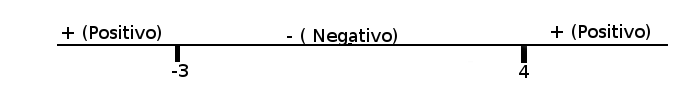
\includegraphics[scale=0.53]{imagens/exemplo1IneGrau2.png}
\end{flushleft}
\item Agora observando a imagem acima devemos responder a pergunta que a inequação $x^{2} - x - 12 > 0$ nos faz. Qual o momento em que o sinal da inequação está positivo? Se analisar a figura veremos que o sinal se mantem negativo no intervalo de $[-3;4]$, então nosso conjunto solução consiste nos intervalos que mantêm nosa inequação positiva, que são $(-\infty ; -3)\cup(4 ; +\infty)$.
\end{itemize}
\\
\textbf{Exemplo X.X:} Seja a inequação $2x^{2} + 3x \leq 20$, encontre o conjunto solução: 
\\	
\begin{itemize}
\item Primeiramente deve-se colocar todos os termos para um lado afim de deixar a inequação na forma padrão, então;
\item[] $2x^{2} + 3x -20 \leq 0$
\item Visualizando a inequação formada, ja temos os elementos para realizar a Bhaskara sendo $a = 2$, $b = 3$ e $c = -20$, então:
\begin{center}
\item[] $\frac{-3 \pm \sqrt{3^{2} - 4.2.(-20)}}{2.2} \Rightarrow \frac{-3 \pm 13}{4}$
\item[] $\frac{-3 \pm 13}{4} \Rightarrow =\left\{\begin{array}{rc} x' = -4,&\mbox{}\quad \frac{-3-13}{4},\\ x'' = 5/2, &\mbox{}\quad  \frac{-3+13}{4} .
\end{array}\right$
\end{center}
\item Sabemos que a inequação é positiva com concavidade para cima pois $a > 0$, então vamos colocar as informações disponíveis na regra e obter o conjunto solução correto:
\begin{flushleft}
	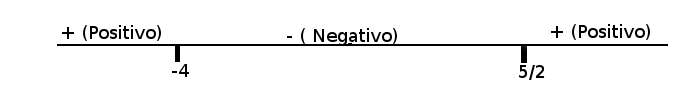
\includegraphics[scale=0.53]{imagens/exemplo2IneGrau2.png}
\end{flushleft}
\item Por fim vamos realizar o mesmo questionamento sobre a inequação $2x^{2} + 3x -20 \leq 0$, lembrando que essa análise sempre é feita com a inequação desigualada a zero. Então observando o simbolo $\leq$ a inequação quer em qual intervalo num´erico os valores obtidos são sempre menores ou iguais a zero? A resposta se obtem analisando a tabela $[-4 ; 5,2]$, observando que o intervalo é fechado pois os zeros da inequação estão sendo requeridos pela inequação.
\end{itemize}
\\
\textbf{Exemplo X.X:} Seja a inequação $-x^{2} +20 \leq -5$, encontre o conjunto solução: 
\\	
\begin{itemize}
\item Vamos colocar todos os termos para o lado esquerdo da desigualdade e deixar o zero do lado direito, assim:
\begin{center}
\item[]$-x^{2} +25 \leq 0$
\end{center}
\item O fato de realizar o passo anterior, irá facilitar na analise após todos os cálculos serem feitos, neste ponto podemos utilizar a Bhaskara, porém existe outro modo de fazer esta resolução. Como trata-se da existência de somente um x e este de grau 2, podemos inferir o resultado diretamente da seguinte maneira:
\begin{center}
\item[] $-x^{2} \leq -25 \Rightarrow x^{2} \geq 25 \Rightarrow x \geq \sqrt{25} \Rightarrow x \geq \pm 5$
\end{center}
\item Assim sabemos nossas raízes que são $x' = -5$ e $x'' = 5$. Agora vamos criar a tabela de an´alise:
\begin{flushleft}
	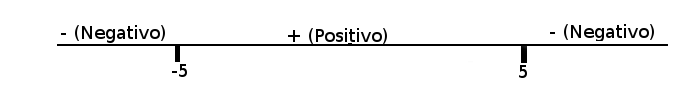
\includegraphics[scale=0.53]{imagens/exemplo3IneGrau2.png}
\end{flushleft}
\item Observando a imagem a seguir e conjuntamente a inequação desigulada a zero $-x^{2} +25 \leq 0$, em que momento a inequação obtem números menores ou iguais a zero? O conjunto solução é $(-\infty ; -5]\cup[5 ; +\infty)$. Para fins de certificação, incentivamos o leitor a resolver a mesma inequação utilizando o método da Bhaskara.
\end{itemize}

\\
\textbf{Exemplo X.X:} Seja a inequação $x^{2} - 10x > 0$, encontre o conjunto solução: 
\\	
\begin{itemize}
\item Para este exemplo utilizaremos outro método mais rapido de se realizar uma analise de inequação, como nossa ja esta desigualda a zero, podemos ver que do lado esquerdo existe um fator comum entre os dois termos que é o $x$. Vamos simplificar essa inequação:
\begin{center}
\item[] $x^{2} - x < 0 \Rightarrow x(x - 10) < 0 $
\end{center}
\item A partir deste ponto podemos separar a inequação em dois casos, em que cada caso consiste em uma equação das partes da inequação:
\item[\textbf{Caso 1}] $x = 0$ ja é uma das raízes da equação $x' = 0$, então neste caso ja esta feita todas as operações possíveis ;
\item[\textbf{Caso 2}] $x - 10 = 0 \Rightarrow x = 10$, nossa segunda raiz então é $x'' = 10$
\item Observando a tabela de análise, vamos introduzir as raízes descobertas e descobrir a solução: 
\begin{flushleft}
	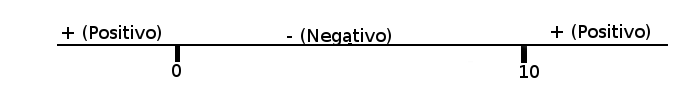
\includegraphics[scale=0.53]{imagens/exemplo4IneGrau2.png}
\end{flushleft}
\item Sabendo que $a > 0$, e respondendo a desigualdade da inequação $x^{2} - 10x > 0$ temos como conjunto solução o intervalo $(-\infty ; 0)\cup(10 ; +\infty)$.
\end{itemize}

%%%%%%%%%%%%%%%%%%%%%%%%%%%%%%%%%%%%%%END INEQUACOES%%%%%%%%%%%%%%%%%%%%%%%%%%%%%%%%%%%% 


%%%%%%%%%%%%%%%%%%%%%%%%%%%%%% FUNÇÕES %%%%%%%%%%%%%%%%%%%%%%%%%%%%%%%%%%%%%%%%%%%%%%%%%
\chapter{Funções}
As funções se enquadram em um dos assuntos mais importantes da matemática, onde a maior parte das aplicações e teorias desenvolvidas contenham as funções em sua síntese. Uma função corresponde a associação de elementos de um conjunto a elementos de outro conjunto. Também deve-se enfatizar que uma função é deterministica, ou seja, dada uma entrada o resultado sempre será coerente com esta entrada. Todos os conjuntos que iremos trabalhar sempre serão subconjuntos de $\Re$ e o par de conjuntos trabalhado sempre será retratado por um par ordenado (x,y).

\section{Definição}
Sejam A e B subconjuntos de $\Re$. Uma função $f$:A $\rightarrow$ B é uma lei ou regra de cada elemento de A faz corresponder um \textbf{único} elemento de B. O conjunto A é chamado de \textit{domínio} de $f$ e o conjunto B é chamado de \textit{contradomínio}.\\
\begin{itemize}
\item $f$:A $\rightarrow$ B
\item $x \rightarrow f(x) $
\end{itemize}
\\
\textbf{Exemplo X.X:} Sejam dois conjuntos A = $\{$2,4,5$\}$ e B = $\{$10,20,25$\}$. Realize o mapeamento da função $f(x):5x$
\\
\begin{center}
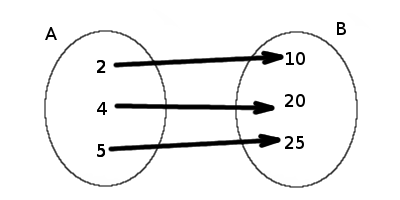
\includegraphics[scale=0.6]{imagens/conjuntoExFunc1.png}
\end{center}
Como foi introduzido antes, toda função e uma associacao de elementos do conjunto A com o seu correspondendo no conjunto B e pode ser representada essa associação através de pares ordenados. Os pares deste exemplo correspondem (2,10) , (4,20) , (5,25).
\\
\\
\textbf{Contra-Exemplo X.X:} Sejam dois conjuntos A = $\{$2,4,5$\}$ e B = $\{$10,20,25$\}$. A os conjuntos abaixo não correspondem a uma função.
\\
\begin{center}
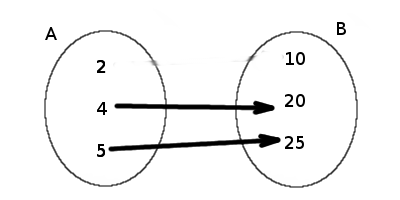
\includegraphics[scale=0.6]{imagens/conjuntoExFunc2.png}
\end{center}
\\
Não corresponde uma função pois o elemento 3 esta associado a dois elementos diferentes do conjunto B, o que nao satisfaz as condições de função.
\\
\begin{itemize}{}
\item Para cada elemento do domínio somente pode ter um correspondente do contradomínio, ou seja, $x \in A$ e $y \in B$, ent'ao $f(x) = x$ ou pode ser denotado também por $ y = x$.
\item O conjunto de elementos que são assoaciados pelo elementos do conjunto domínio, podemos também chama-los de conjunto imagem.
\item Toda função tem somente uma regra que a define para todos os elementos do domínio, tornando-a determinística.
\item Toda função contem um gráfico, no qual e definido por todos os seus pontos resultantes.
\end{itemize}

\section{Gráfico}
Podemos associar a cada par que compôem a função um ponto em um sistema de eixos coordenados. O sistema mais comum é composto por um eixo horizontal e um eixo vertical que se cruzam na origem(0,0).\\
O primeiro elemento do par é associado a um ponto no eixo horizontal e o segundo elemento é associado a um ponto no eixo vertical.\\
O encontro das paralelas aos eixos por esses pontos define a representação gráfica do par funcional.
\\
\textbf{Exemplos de Gráficos:}
\begin{center}
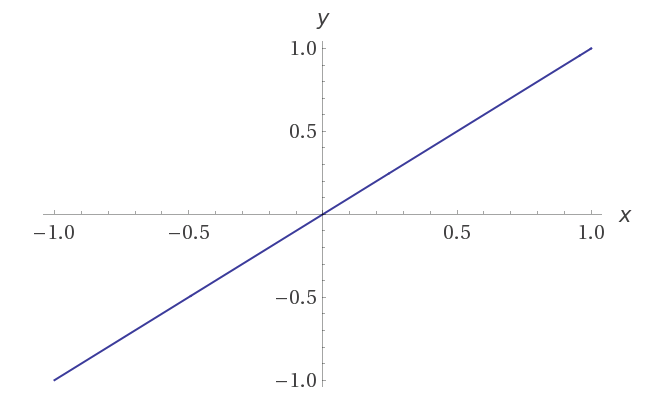
\includegraphics[scale=0.3]{imagens/plot1.png}
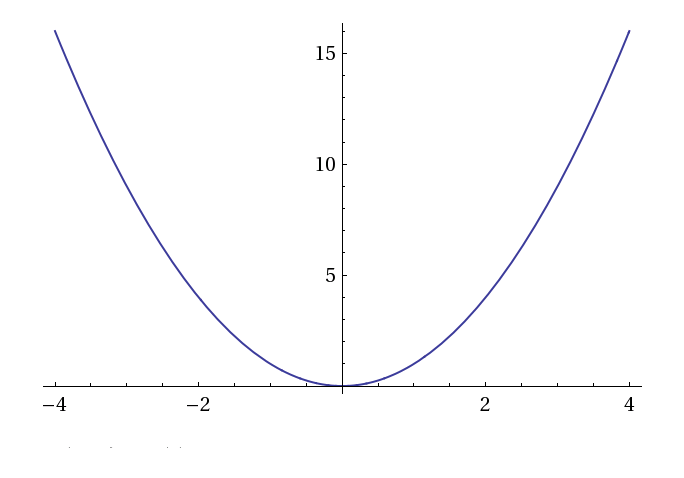
\includegraphics[scale=0.3]{imagens/plot2.png}
\end{center}
\\
Sabemos que cada função contêm uma regra quanto a determinação de seus pontos dado um valor do conjunto domínio. Essas regras são os fatores delimitantes para a criação dos gráficos acima. Porem existem muitos modos de se criar gráficos, seja conhecendo a forma de grandeza da função ou realizando o método da substituição de cada ponto do domínio na função, afim de encontrar seus pontos no gráfico. Vejamos alguns exemplos de construção de gráfico.
\\
\\
\textbf{Exemplo X.X}: Consideramos a função $f(x) = x + 1$. Monte o gráfico a partir do intervalo [-2 ; 8). Determine o domínio e a imagem deste gráfico:
\begin{center}
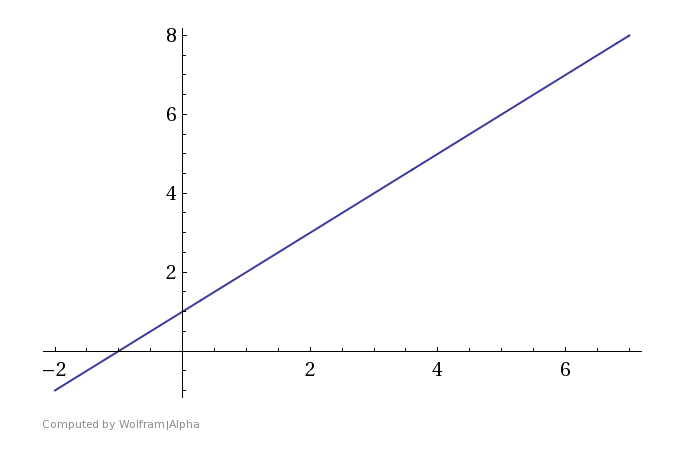
\includegraphics[scale=0.3]{imagens/plot3.png}
\end{center}
\\

\textbf{Exemplo X.X}: Vejamos o gráfico da função $f(x) = |x|$. Como vimos anteriormente na seção X.X(valor absoluto):\\
\begin{center}
$|x| =\left\{\begin{array}{rc}
x,se &\mbox{}\quad x \geq 0,\\
-x,se &\mbox{}\quad x < 0 .
\end{array}\right
$
\end{center}
\\
\begin{center}
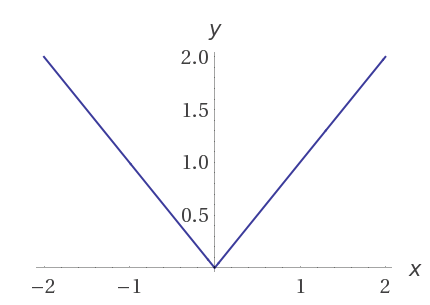
\includegraphics[scale=0.5]{imagens/plot4.png}
\end{center}
\\
Então a partir disto temo uma função com duas condicoes para cálculo. Caso o valor a ser calculado seja maior que 0 então sera calculado atraves da $f(x) = x$, caso o valor seja menor que zero, então a regra a ser utilizada é $f(x) = -x$. As funções podem ser intercaladas, afim de ter varias funções que são utilizadas a partir de um determinado intervalo de valores. \\

\subsubsection{Operações:}
Assim como podemos adicionar, subtrair, multiplicar e dividir números, também podemos produzir novas funções através de operações. Estas operações são definidas como segue:
\\
\begin{enumerate}
Sejam $f$ e $g$ duas funções distintas, temos as operações básicas:
\item $(f + g)(x) = f(x) + g(x)$
\item $(f - g)(x) = f(x) - g(x)$
\item $(f . g)(x) = f(x) . g(x)$
\item $(f / g)(x) = \frac{f(x)}{g(x)}$
\end{enumerate}
O domínio das funções $f+g$, $f-g$ e $f.g$ é a intersecção dos domínios de f e g. O domínio de $\frac{f}{g}$ é a intersecção dos domínios de f e g, excluindo-se os pontos x onde $g(x) = 0$.

\section{Funções Importantes}
Uma função pode ser criada para diversos fins, outras são destinadas a resolver problemas específicos. Porém algumas destas funções são de extrema importância, uma vez que estão ligadas a maioria dos problemas existentes. São elas:

\subsection{Função Linear}
É uma função definida em $\Re$ e dada pela regra $f(x) = ax + b$, onde a e b são números reais. O gráfico de uma função linear é uma reta, pois ela tem variação constante, dada pelo valor de a. Os números a e b, são chamados respectivamente de coeficiente angular e linear.\\
Quando $a > 0$ a função $f(x) = ax + b$ é crescente, isto é, à medida que x cresce, f(x) também cresce. Quando $a<0$ a função $f(x) = ax + b$ é descrescente, isto é, à medida que x cresce, $f(x)$ decresce.
\\
\textbf{Gr´aficos}
\\
\begin{center}
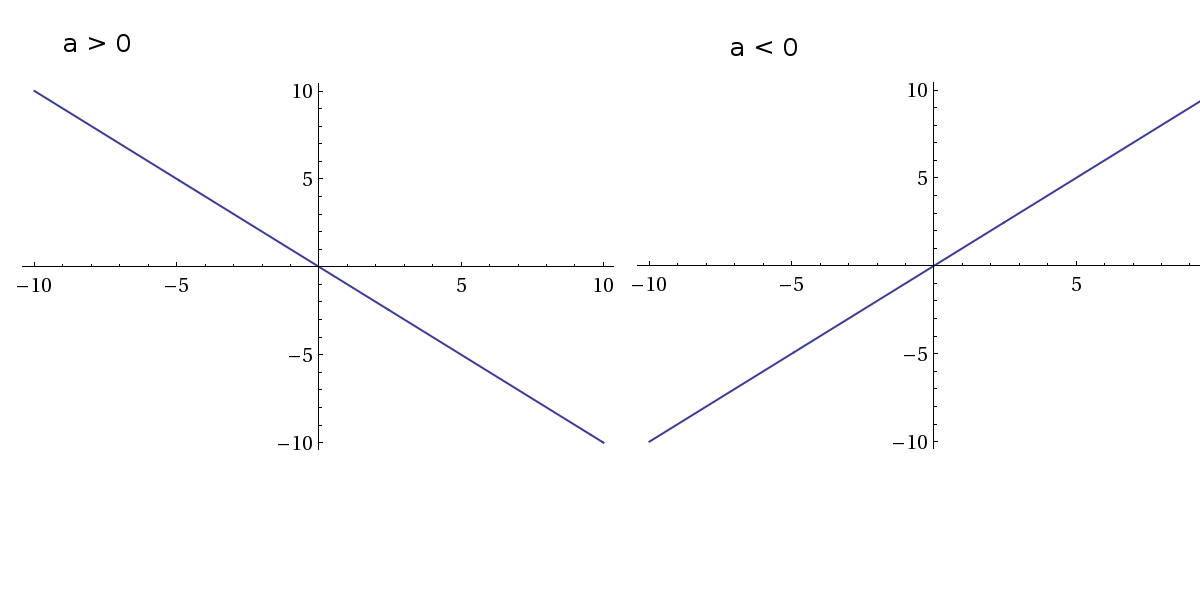
\includegraphics[scale=0.3]{imagens/plot5.png}
\end{center}
\textbf{Exemplo X.X}: Dado a função $f(x) = -5x + 10$, indique seu domìnio e construa seu gráfico:
\\
\begin{itemize}
\item Primeiramente, para podermos definir o ponto que a reta intersecta o eixo x, devemos igualar a função a zero. E juntamente com este passo veremos como sera o domínio.
\item Observando o número o coeficiente angular, notamos que ele é menor que zero, então trata-se de uma função decrescente.
\item $f(x) = -5x + 10$, então temos:
\begin{center}
$-5x + 10 = 0$\\
$-5x = -10$\\
$5x = 10$\\
$x = 2$
\end{center}
\item Vemos o gráfico cruzara o eixo x no ponto 2, ou seja, quando x for dois a função zera 0.
\item Vejamos o gráfico desta função:
\begin{center}
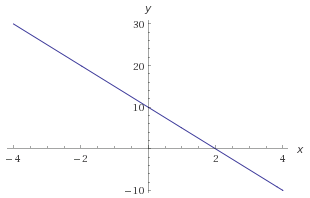
\includegraphics[scale=0.8]{imagens/plot6.png}
\end{center}
\end{itemize}
\subsection{Função Quadrática}
É uma função dada pela regra $f(x) = ax^{2} + bx + c$. com domínio em $\Re$, onde a,b e c são números reais e $a \neq 0$.\\O gráfico de uma função quadrática é modelado através de uma parábola que assume diversas posições dependendo do sinal do coeficiente angular. Essas posições da parábola foram apresentadas na seç~ao de \textbf{Inequações de Segundo Grau}. Vejamos alguns exemplos:
\\
\\
\textbf{Exemplo X.X}: Dado a função $f(x) = x^{2} - 5x + 6$, construa seu gráfico: 
\begin{itemize}
\item Primeiramente, seguindo as regras de ordem da função, vemos que o coeficiente angular é positivo o que indica que a parábola esta voltada para cima;
\item Como era feito nas inequações, deve-se igual a função a zero afim de descobrir os pontos que cruzam o eixo.
\begin{center}
$f(x) = x^{2} - 5x + 6$\\
$0 = x^{2} - 5x + 6$\\
$\frac{5 \pm \sqrt{(-5)^{2} - 4.1.6}}{1.2}$\\
$\frac{5 \pm \sqrt{1}}{2}$\\
$\frac{5 \pm 1}{2}$\\
$x' = 3$ e $x'' = 2$
\end{center}
\item Temos que os valores que interectam o eixo x são 3 e 2, sabendo disso vejamos como ficará o gráfico:
\begin{center}
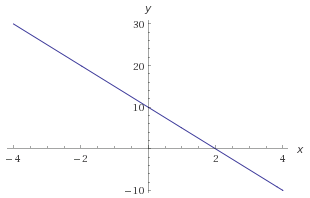
\includegraphics[scale=0.8]{imagens/plot6.png}
\end{center}
\end{itemize}

\subsection{Função Racional}
É função definida como o quociente de duas funções polinimiais, isto é, $f(x) = \frac{f(x)}{g(x)}$ onde $g(x) \neq 0$. O seu domínio corresponde todos $\Re$ exceto os que tornam $g(x) = 0$.
\\
\textbf{Exemplo X.X}: Dado a função $f(x) = \frac{x - 1}{x + 1}$, construa seu gráfico: 
\begin{itemize}
\item Primeiramente devemos achar o ponto em que o$g(x)$ intersectaria a reta, uma vez que este ponto não pode existir;
\begin{center}
$x+1 = 0$\\
$x = -1$
\end{center}
\item Sabemos a partir disto que o domínio é $\Re - {-1}$ pois o valor -1 para x, torna função indeterminável. Vejamos como é o gráfico desta função;
\begin{center}
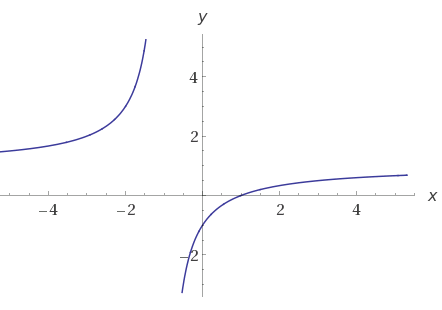
\includegraphics[scale=0.5]{imagens/plot8.png}
\end{center}
\end{itemize}

\subsection{Função Par e Impar}
As funções pares e impares são alguns casos especiais de funções. Uma função denominada par é relacionada aos elementos introduzidos na função, ou seja, seja todos os valores possiveis no domínio de $f, f(-x) = f(x)$, isto quer dizer que não importanto o sinal do x, o seu valor manterá sempre o mesmo.\\
Ja a função impar possui exeplificação contraria a das funções pares, dado uma função $f(x)$ digamos que ela é impar se todos os elementos do domínio de $f, f(-x) = -f(x)$.\\
\\
\textbf{Exemplos X.X} 
\begin{itemize}
\item A funç~ao $f(x) = x^{2}$, é par, ja que $f(-x) = (-x^{2}) = x^{2} = f(x)$;
\item A funç~ao $f(x) = x^{5} + x^{3}$ é impar, ja que $f(-x) = (-x^{5}) + (x^{3}) = -f(x)$;
\item A funçao $f(x) = x^{3} + 4$ não é par nem impar. 
\end{itemize}

\begin{center}
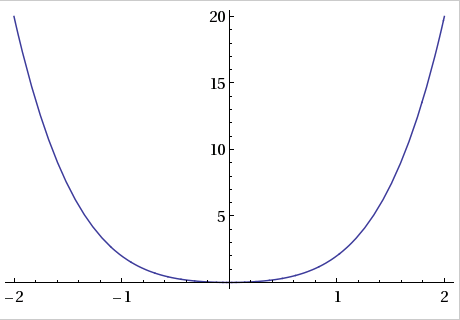
\includegraphics[scale=0.5]{imagens/plotPar.png}
\end{center}

\subsection{Função Exponencial}
Chama-se de função exponencial de base $a$, a função f de $\Re$ em $\Re$ que associa a cada $x$ real o número real $a^{x}$, sendo a um número real, $0 < a \neq 1$. O domínio desta função é considerado nos $\Re$ e sua imagem é $(0 ; +\infty)$.

\begin{itemize}
\item A curva que o representa está toda acima do eixo das abscissas, pois $a^{x} > 0 \forall x \in \Re$;
\item Corta o eixo das ordenadas no ponto (0,1);
\item $f(x) = a^{x}$ é crescente se a > 1 e descrescente se 0 < a < 1.
\end{itemize}

\begin{center}
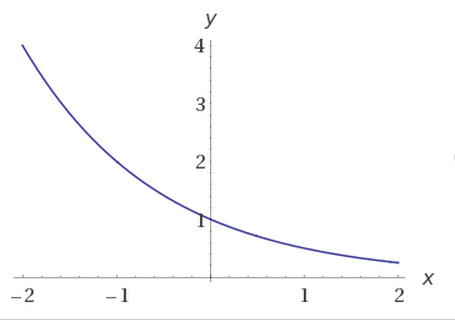
\includegraphics[scale=0.5]{imagens/plotExponencial.png}
\end{center}

\subsection{Função Logarítmica}
Da um número real a ($0 < a \neq 1)$, chamamos de função logarítmica de base a entre $(0;+\infty)$ que associa a cada $x$ o número $\log_{a}x$. Então $f(x) = \log_{a}x$.

\begin{center}
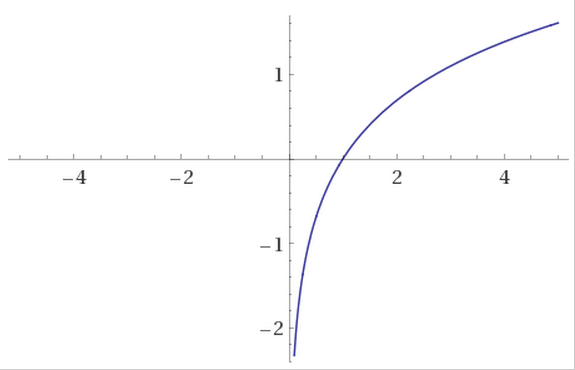
\includegraphics[scale=0.5]{imagens/plotLogartim.png}
\end{center}

\begin{itemize}
\item Está todo a direta do eixo y;
\item Corta o eixo das abscissas no ponto (1,0);
\item $f(x) = \log_{a}x$ é crescente se $a > 1$ e descrescente se $0 < a < 1$;
\end{itemize}

\section{Funções Trigonométricas}

\begin{center}
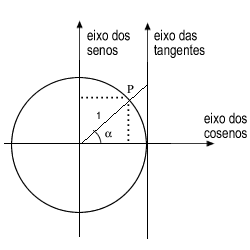
\includegraphics[scale=0.8]{imagens/Trigonometry.png}
\end{center}
\subsection{Função Seno}
Seja $x$ um número real. Marcamos um ângulo com medida $x$ radianos, na circunferência unitária com centro na origem. Seja P o ponto de intersecção do lado terminal do ângulo $x$, com essa circunferência.
\\
Definimos a função seno como a função $f$ de $\Re$ em $\Re$ que a cada $x \in \Re$ faz corresponder o n´umero real $f(x) = sen x$. O domínio desta função corresponde aos $\Re$ e a imagem consiste no intervalo de [-1;1]. Vejamos abaixo o gráfico da função seno:

\begin{center}
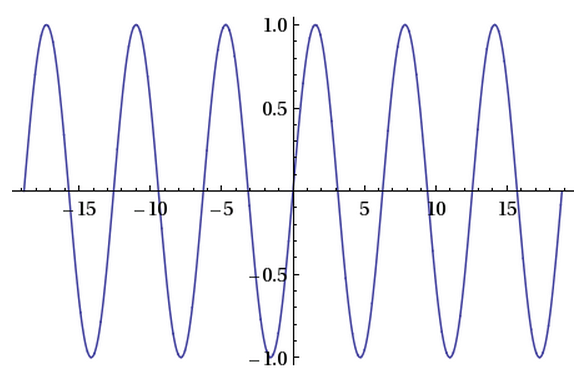
\includegraphics[scale=0.5]{imagens/plotSeno.png}
\end{center}

\subsection{Função Cosseno}
Seja $x$ um número real. Denominamos cosseno de $x$ a abcissa OP_{2} do ponto P em relação ao sistema U O V, Definimos a função cosseno como a função $f$ de $\Re$ em $\Re$ que a cada $x \in \Re$ faz corresponder o número real $f(x) = cos x$. O domínio da função cosseno é $\Re$ e o conjunto imagem corresponde ao intervalo [-1;1]. Vejamo como fica a variação da função cosseno.

\begin{center}
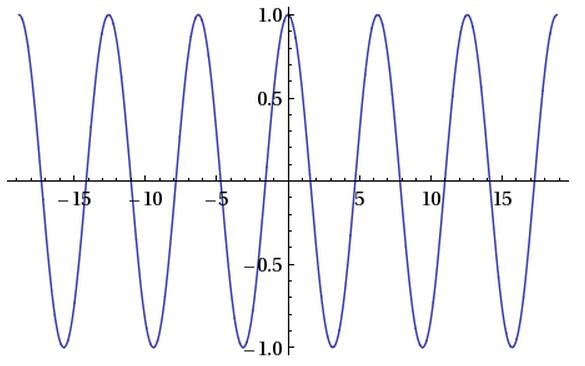
\includegraphics[scale=0.5]{imagens/plotCos.png}
\end{center}

\subsection{Função Tangente}
A função tangente é uma composição entre as duas funções trigonométricas abordadas antes, então a função tangente é definida como $f(x) = Tg x \Rightarrow f(x) = \frac{Sen x}{Cos x}$. A seguir o gráfico da função tangente.

\begin{center}
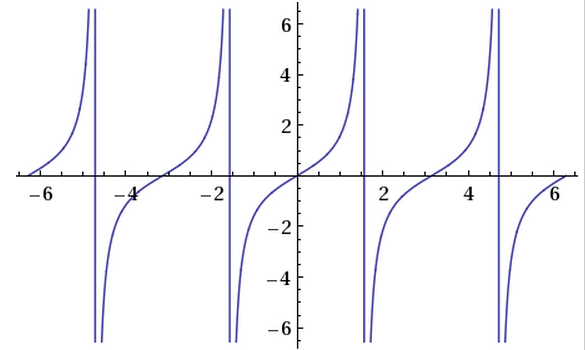
\includegraphics[scale=0.5]{imagens/plotTan.png}
\end{center}

%%%%%%%%%%%%%%%%%%%%%%%%%%%%%%%%END FUNÇÕES%%%%%%%%%%%%%%%%%%%%%%%%%%%%%%%%%%%%%%%%%%%%

\chapter{References}

\appendix
\renewcommand{\chaptername}{Appendix}

\end{document}